\documentclass{amsart}
\usepackage{amsmath,amssymb,amsthm,amsfonts,amscd,mathrsfs,mathtools}
\usepackage[utf8]{inputenc}
\usepackage{graphicx}
\usepackage[hyphens]{url}
\usepackage{caption}
\usepackage{hyperref}
\usepackage{tikz-cd}



\theoremstyle{plain}
    \newtheorem{thm}{Theorem}[section]
    \newtheorem{lem}[thm]   {Lemma}
    \newtheorem{cor}[thm]   {Corollary}

\theoremstyle{definition}
    \newtheorem{defn}[thm]  {Definition}
    \newtheorem{conj}[thm]{Conjecture}

\newcommand{\C}{\mathbb{C}}
\newcommand{\cC}{\mathfrak{C}}
\newcommand{\fc}{\mathfrak{c}}
\newcommand{\D}{\mathcal{D}}
\newcommand{\F}{\mathbb{F}}
\newcommand{\cF}{\mathcal{F}}
\renewcommand{\H}{\mathcal{H}}
\newcommand{\M}{\mathcal{M}}
\newcommand{\N}{\mathcal{N}}
\newcommand{\p}{p}
\newcommand{\cP}{\mathcal{P}}
\newcommand{\Q}{\mathbb{Q}}
\newcommand{\R}{\mathbb{R}}
\renewcommand{\S}{\mathcal{S}}
\newcommand{\fS}{\mathfrak{S}}
\newcommand{\T}{\mathcal{T}}
\newcommand{\U}{\mathcal{U}}
\renewcommand{\u}{\mathfrak{u}}
\newcommand{\V}{\mathcal{V}}
\renewcommand{\v}{\mathfrak{v}}

\newcommand{\Z}{\mathbb{Z}}


\newcommand{\sgm}{\Sigma_{g,1}^m}
\newcommand{\sg}{\Sigma_{g,1}}

\newcommand{\Sg}{\mathcal{S}_{g,1}}
\newcommand{\Sgm}{\Sg^m}

\newcommand{\mg}{\mathfrak{M}_{g,1}}
\newcommand{\mgm}{\mg^m}
\newcommand{\Ig}{\mathcal{I}_{g,1}}

\renewcommand{\gg}{\Gamma_{g,1}}
\newcommand{\ggm}{\gg^m}

\newcommand{\bms}{\beta_{m}(\sg)}
\newcommand{\fms}{F_m(\sg)}
\newcommand{\cms}{C_m(\S)}
\newcommand{\fmsD}{C_{1,m}^{\D}(\S)}
\newcommand{\cmsD}{C_{m}^{\D}(\S)}
\newcommand{\fmstwoD}{C_{1,m}^{(2),\D}(\S)}
\newcommand{\cmstwoD}{C_{m+1}^{(2),\D}(\S)}
\newcommand{\Dmone}{\triangle_{m+1}}
\newcommand{\Donem}{\triangle_{1,m}}
\renewcommand{\i}{\iota}
\renewcommand{\j}{j}
\newcommand{\pr}{\mathfrak{p}}

\newcommand{\symb}{\mathcal{S}}
\newcommand{\bsymb}{\bar\symb}
\newcommand{\tup}{\mathfrak{h}}

\newcommand{\bH}{\mathbb{H}}
\newcommand{\cH}{\mathcal{H}}

\newcommand{\Ch}{\mathcal{C}}
\newcommand{\tCh}{\tilde\Ch}
\newcommand{\tH}{\tilde{H}}

\newcommand{\ZcC}[1]{\Z_2\left<\cC^{#1}\right>}
\newcommand{\tpsi}{\tilde\psi}

\newcommand{\pa}[1]{\left(#1\right)}
\newcommand{\qua}[1]{\left[#1\right]}
\newcommand{\abs}[1]{\left|#1\right|}
\newcommand{\set}[1]{\left\{#1\right\}}

\newcommand{\Sone}{\mathbb{S}^1}
\newcommand{\mrS}{\mathring{\S}}
\newcommand{\gone}{\Gamma_{1,1}}
\newcommand{\tu}{\tau_{\u}}
\newcommand{\tv}{\tau_{\v}}

\newcommand{\ux}{\underline{x}}
\newcommand{\uu}{\underline{u}}
\newcommand{\uv}{\underline{v}}
\newcommand{\ualpha}{\underline{\alpha}}

\newcommand{\tildeu}{\tilde u}
\newcommand{\tildev}{\tilde v}

\newcommand{\SP}{S\!P}

\renewcommand{\phi}{\varphi}
\renewcommand{\epsilon}{\varepsilon}

\newcommand{\hor}{hor}
\newcommand{\ver}{ver}

\renewcommand{\L}{\Lambda}
\DeclareMathOperator{\Diff}{Diff}
\DeclareMathOperator{\Imm}{Imm}
\DeclareMathOperator{\rk}{rk}
\DeclareMathOperator{\Ker}{ker}
\DeclareMathOperator{\coker}{coker}
\DeclareMathOperator{\Sym}{Sym}
\DeclareMathOperator{\Id}{Id}
\DeclareMathOperator{\Hom}{Hom}


\DeclarePairedDelimiter\ceil{\lceil}{\rceil}
\DeclarePairedDelimiter\floor{\lfloor}{\rfloor}
\def\colim{\mathop{\mathrm{colim}}\nolimits}
    
\begin{document}

\title{Splitting of the homology of the punctured mapping class group}

\author{Andrea Bianchi}

\address{Mathematics Institute,
University of Bonn,
Endenicher Allee 60, Bonn,
Germany
}



\email{bianchi@math.uni-bonn.de}

\date{\today}


%\keywords{Topological complexity, aspherical spaces, Lusternik-Schnirelmann category, cohomological dimension, topological robotics, braid groups}
%\subjclass[2010]{55M99, 55P20 (Primary); 55M30, 20J06, 68T40 (Secondary).}

\begin{abstract}
Let $\ggm$ be the mapping class group of an orientable surface $\sgm$ of genus $g$ with one parametrised
boundary component and $m$ permutable punctures, and let $\bms$ be the braid group on $m$ strands
of the surface $\sg$. We prove that $H_*(\ggm;\Z_2)\cong H_*(\gg;H_*(\bms;\Z_2))$.
We compute (?) the right hand side explicitly for $g=1$.
\end{abstract}

%\thanks{}

\maketitle

\section{Introduction}
Let $\sg$ be a smooth orientable surface of genus $g$ with one boundary curve $\partial\sg$, and let $\sgm$ be $\sg$ with
a choice of $m$ distinct points in the interior, called \emph{punctures}.

Let $\gg$ be the mapping class group of $\sg$, i.e. the group of isotopy classes of diffeomorphisms of $\sg$:
diffeomorphisms are required to fix $\partial\sg$ pointwise. Similarly let $\ggm$ be the mapping class group of $\sgm$, i.e.
the group of isotopy classes of diffeomorphisms of $\sgm$ that fix $\partial\sgm$ pointwise and \emph{permute} the $m$ punctures.

Forgetting the punctures gives a surjective map $\ggm\to\gg$ with kernel $\bms$,
the $m$-th \emph{braid group} of the surface $\sg$. We obtain the Birman exact sequence (see \cite{Birman:mcgbr})
\begin{equation}
\label{eq:Birman}
1\to\bms\to\ggm\to\gg\to 1.
\end{equation}
% This short exact sequence corresponds to 
% \begin{equation}
%  \cms\to\mgm\to\mg.
% \end{equation}
% Here $\cms$ is the \emph{unordered} configuration space of $m$ points in the interior of $\Sigma$, i.e.
% \begin{equation}
%  \cms=\fms/\S_m=\set{(p_1,\dots,p_m)\in\pa{\mathring\sg}^m|p_i\neq p_j \;\forall i\neq j}/\S_m,
% \end{equation}
% the quotient of the \emph{ordered} configuration space of $m$ points in the interior of $\Sigma$ by the natural
% action of the symmetric group $\S_m$ that permutes the (ordered list of) points in the configuration; $\mg$ and $\mgm$
% are the moduli spaces of Riemann structures on $\sg$ and $\sgm$ respectively.

The associated Leray-Serre spectral sequence $E(m)$ in $\Z_2$-homology has a second page $E(m)^2_{k,q}=H_k(\gg;H_q(\bms;\Z_2))$,
and converges to $H_{k+q}(\ggm;\Z_2)$.

The main result of this article is that this spectral sequence collapses in its second page.
\begin{thm}
\label{thm:main}
For all $l\geq 0$ there is an isomorphism of vector spaces
\begin{equation}
\label{eq:main}
H_l\pa{\ggm;\Z_2}\cong \bigoplus_{k+q=l} H_k\pa{\gg;H_q\pa{\bms;\Z_2}}.
\end{equation}
\end{thm}
Thus the computation of $H_*\pa{\ggm;\Z_2}$ reduces to the computation of the homology of $\gg$ with
twisted coefficients in the representation $H_*\pa{\bms;\Z_2}$. We will see that this $\gg$-representation
splits as a direct sum of symmetric powers of $H_1(\sg)$ with the symplectic action: this is done in
Theorem \ref{thm:Hbms*as*ggrep}, which together with Theorem \ref{thm:main} is the main result of the article.
% in section \ref{sec:HBraidSurf}).

%In particular this representation is symplectic: this had already benn stated in \cite{LM}.

% The group $\gg$ is significantly smaller than $\ggm$, so the
% computation of the right-hand side of equation \eqref{eq:main}
% may be more tractable.
%WE DO THIS COMPUTATION FOR $g=1$.

The strategy of the proof does not generalize to fields of characteristic different from 2 or to the \emph{pure}
mapping class group, in which we consider only diffeomorphisms of $\sgm$ that fix all punctures. In section \ref{sec:rational}
we describe in detail a counterexample with coefficients in $\Q$, which can be generalized both to coefficients
in a field $\F_p$ of odd characteristic and to the pure mapping class group.

I would like to thank my PhD advisor Carl-Friedrich B\"odigheimer for his precious suggestions and his continuous encouragement
during the preparation of this work.

\section{Preliminaries}
\label{sec:Preliminaries}
In the whole article $\Z_2$-coefficients for homology and cohomology will be understood,
unless explicitly stated otherwise.

In this section we recollect some classical definitions and results about braid groups and mapping class groups.
Let $\sg$ be a compact, smooth, orientable surface of genus $g$ with one parametrised
boundary component $\partial \sg$. Let $\sgm$ be $\sg$ with a choice of $m$ distinct
points in the interior: these points are called \emph{punctures} and are not assumed to be ordered.

\begin{defn}
\label{defn:cms}
 The $m$-th \emph{ordered configuration space} of a surface $\sg$ is the space
\[
 F_m(\sg)=\set{(P_1,\dots,P_m) \in \pa{\mathring{\Sigma}_{g,1}}^{\times m}  \,|\,  P_i\neq P_j  \;\forall i\neq j}.
\]

 Notice that we require the points of the configuration to lie in the interior of $\sg$;
 $F_m(\sg)$ is a smooth, orientable $2m-$dimensional manifold.
 
 The symmetric group $\mathfrak{S}_m$ acts freely on $F_m(\sg)$ by permuting the points of a configuration;
 the orbit space
 \[
 F_m(\sg)/\mathfrak{S}_m
 \]
 is called the \emph{$m-$th unordered configuration space}
 of $\sg$ and is denoted by $C_m(\sg)$; this space is also a $2m-$dimensional orientable manifold
 (see figure \ref{fig:unordered}).
 
%  
%  We denote by $C_k(\sg)^c$ the one-point compactification of the space $C_k(\sg)$; the point
%  at infinity is denoted by $*$ and serves as basepoint.
\end{defn}

\begin{figure}\centering
 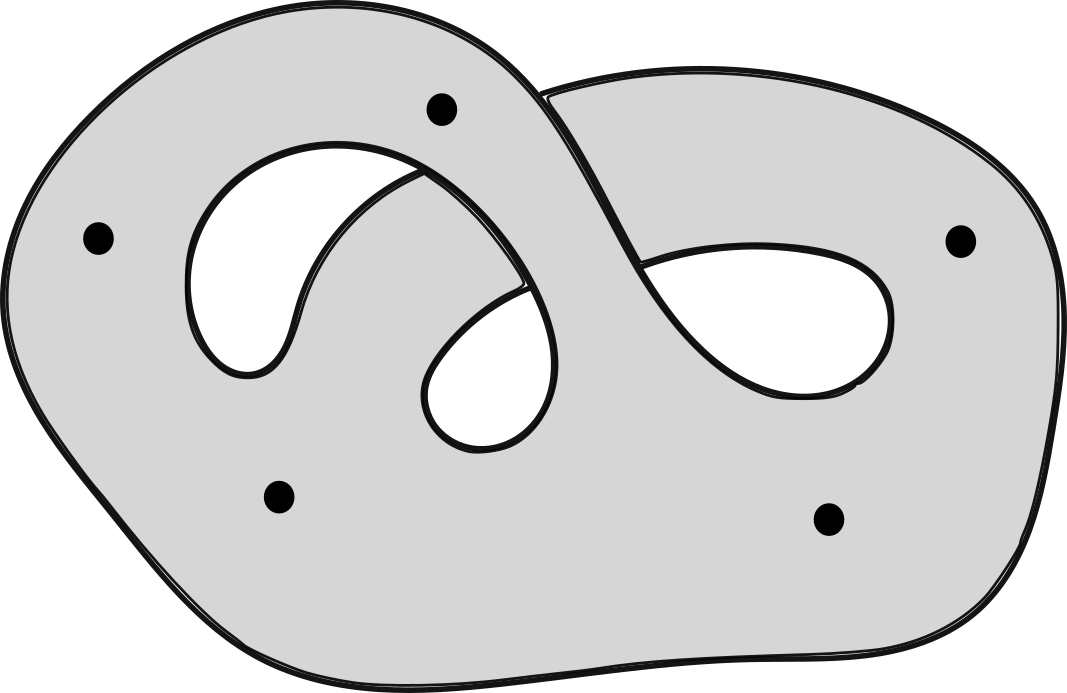
\includegraphics[scale=0.8]{figures/unordered.png}
 \caption{A configuration in the space $C_5(\Sigma_{1,1})$}
\label{fig:unordered}
\end{figure}


A classical result by Fadell and Neuwirth (\cite{FadellNeuwirth}) ensures
that $C_m(\sg)$ is aspherical; the fundamental group $\pi_1(C_m(\sg))$ is
called the \emph{braid group on $m$ strands of $\sg$} and is denoted by $\bms$.

\begin{defn}
 \label{def:mcg}
 Let $\Diff(\sg;\partial\sg)$ be the group of diffeomorphisms of $\sg$ that fix $\partial\sg$ pointwise,
 endowed with the Whitney $C^{\infty}-$topology. We denote by $\gg=\pi_0(\Diff(\sg;\partial\sg))$ its group of connected
 components, which is called the \emph{mapping class group} of $\sg$.
 
 Similarly let $\Diff(\sgm;\partial\sgm)$ be the group of diffeomorphisms of $\sgm$ that fix $\partial(\sg)$
 pointwise and restrict to a permutation of the $m$ punctures, and let $\ggm=\pi_0(\Diff(\sgm;\partial\sgm))$ be its
 group of connected components, called the mapping class group of $\sgm$.
 \end{defn}
 A classical result by Earle and Schatz (\cite{EarleSchatz}) ensures that the connected components
 of $\Diff(\sg)$ are contractible. In particular $B\Diff(\sg;\partial\sg)\simeq B\gg$ is
 a classifying space for
 the group $\gg$, i.e. a space of type $K(\gg,1)$; we call $\cF_{g,1}\to B\Diff(\sg;\partial\sg)$ the universal
 $\sg-$bundle
 \[
  \cF_{g,1}\colon=\sg\times_{\Diff(\sg;\partial\sg)}E\Diff(\sg;\partial\sg)\to B\Diff(\sg;\partial\sg).
 \]
Applying the construction of the $m-$th unordered configuration space fiberwise we obtain a bundle
$C_m(\cF_{g,1})\to B\Diff(\sg;\partial\sg)$ with fiber $C_m(\sg)$.

The space $C_m(\cF_{g,1})$ is a classifying space for the
group $\ggm$ and the Birman exact sequence \ref{eq:Birman} is obtained by taking fundamental
groups of the aspherical spaces
\begin{equation}\label{eq:Birmanbundle}
C_m(\sg)\to C_m(\cF_{g,1})\to B\Diff(\sg;\partial\sg).
\end{equation}

In the whole article the genus $g$ of the surfaces that we consider is supposed to be fixed,
unless explicitly stated otherwise, and we will abbreviate $\S=\sg$.
We denote by $\D$ the open disc $\mathring{\Sigma}_{0,1}$.

It will be useful, for many constructions, to choose an embedding
$\D\hookrightarrow\mrS$ near $\partial\S$ and to replace
$\Diff(\S;\partial\S)$ with its subgroup $\Diff(\S;\partial\S\cup\D)$ of diffeomorphisms
of $\S$ that fix pointwise both $\partial\S$ and $\D$. Saying that $\D$ is embedded
\emph{near $\partial\S$} means that there is a compact subsurface $\S'\subset\S$
such that $\S$ is the boundary connected sum $\S'\natural\bar\D$.
From now on we suppose such an embedding to be fixed and we consider $\D$ as a subspace
of $\mrS$ (see figure \ref{fig:SS'D}). In section \ref{sec:HBraidSurf}, definition \ref{defn:Tsg},
we will specify an embedding $\D\hookrightarrow\mrS$ using a particular model for $\mrS$.

\begin{figure}\centering
 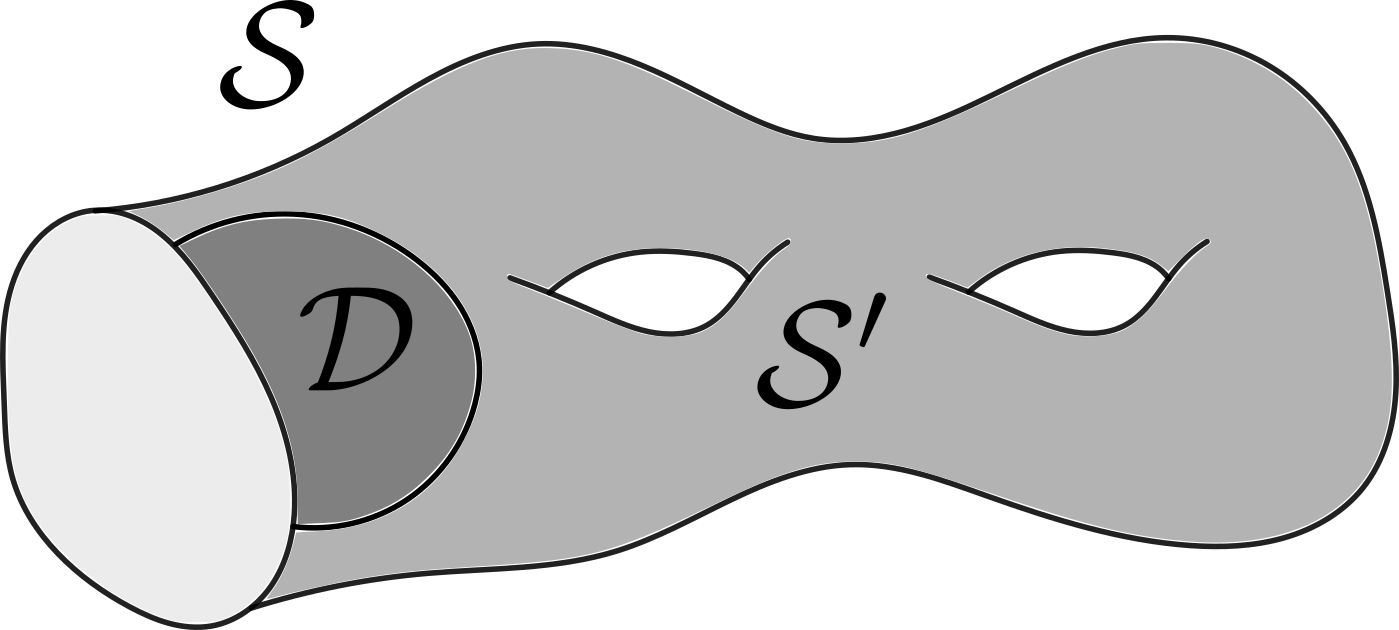
\includegraphics[scale=0.8]{figures/SS'D.png}
 \caption{A splitting of $\S$ as $\S'\natural\bar\D$.}
\label{fig:SS'D}
\end{figure}

The construction of definition \ref{defn:cms} can be specialised to the
surfaces $\D$ and $\S'$, yielding spaces $C_m(\D)$ and $C_m(\S')$ respectively.

The inclusion $\Diff(\S;\partial\S\cup\D)\subset\Diff(\S;\partial\S)$ is a homotopy
equivalence, hence also the induced map
\[
B\Diff(\S;\partial\S\cup\D)\to B\Diff(\S;\partial\S)
\]
is a homotopy equivalence. We will replace the previous construction with the following,
equivalent ones.
\begin{defn}
\label{defn:universalSbundle}
We call $\cF_{\S,\D}\to B\Diff(\S;\partial\S\cup\D)$
the universal $\S-$bundle
 \[
  \cF_{\S,\D}\colon=\S\times_{\Diff(\S;\partial\S\cup\D)}E\Diff(\S;\partial\S\cup\D)\to B\Diff(\S;\partial\S\cup\D).
 \]
Notice that $\Diff(\S;\partial\S\cup\D)$ acts on $\S'$ by restriction of diffeomorphisms, and acts trivially
on $\D$; therefore $\cF_{\S,\D}$ contains subspaces
\[
 \cF_{\S'}= \S'\times_{\Diff(\S;\partial\S\cup\D)}E\Diff(\S;\partial\S\cup\D)
\]
and $\D\times B\Diff(\S;\partial\S\cup\D)$; these subspaces fiber over $B\Diff(\S;\partial\S\cup\D)$
with fibers $\S'$ and $\D$ respectively.

Applying the construction of the $m-$th unordered configuration space fiberwise, we obtain spaces
$C_m(\cF_{\S,\D})$, $C_m(\cF_{\S'})$ and $C_m(\D)\times B\Diff(\S;\partial\S\cup\D)$,
all fibering over $B\Diff(\S;\partial\S\cup\D)$ with fibers, respectively, $\cms$,
$C_m(\S')$ and $C_m(\D)$.
\end{defn}

\begin{defn}
For all $0\leq p\leq m$ there is a natural map
\[
 \mu\colon C_p(\D)\times C_{m-p}(\S')\to \cms
\]
which takes the union of configurations (see figure \ref{fig:defmu}):
 \[
  \mu\pa{\set{P_1,\dots,P_p};\set{P'_1,\dots,P'_{m-p}}}=\set{P_1,\dots,P_p,P'_1,\dots,P'_{m-p}}\in\cms.
 \]
\begin{figure}\centering
 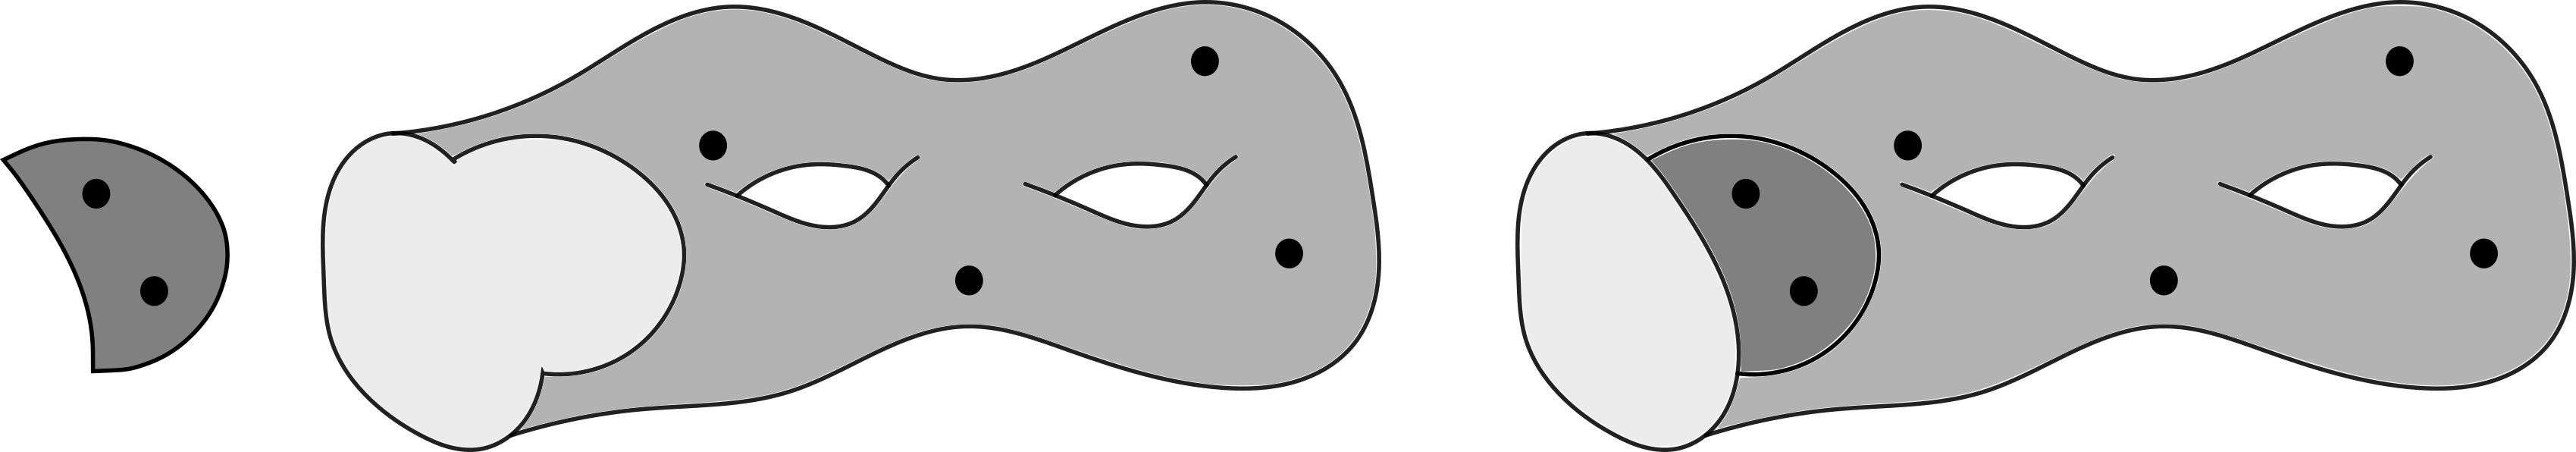
\includegraphics[scale=0.7]{figures/defmu.png}
 \caption{The product of two configurations in $C_2(\D)$ and $C_4(\S)$.}
\label{fig:defmu}
\end{figure}
 
We can apply this construction to each couple of fibers of $C_m(\cF_{\S,\D})$ and $C_{m-p}(\cF_{\S'})$
over the same point of $ B\Diff(\S;\partial\S\cup\D)$, obtaining a map $\mu^{\cF}$:
\[
 \mu^{\cF}\colon C_p(\D)\times C_{m-p}(\cF_{\S'})\to C_m(\cF_{\S,\D}).
\]
If we see the domain of $\mu^{\cF}$ as a fibered product of bundles over $B\Diff(\S;\partial\S\cup\D)$
\[
 \pa{C_m(\D)\times B\Diff(\S;\partial\S\cup\D)}\times_{B\Diff(\S;\partial\S\cup\D)}C_{m-p}(\cF_{\S'}),
\]
then the map $\mu^{\cF}$ is also a map of bundles over $B\Diff(\S;\partial\S\cup\D)$, and the corresponding
map on fibers is precisely $\mu$.
\end{defn}
The fiber bundle \ref{eq:Birmanbundle} corresponding to the Birman exact sequence \ref{eq:Birman}
can now be replaced by the following one
\begin{equation}\label{eq:BirmanbundleD}
\cms\to C_m(\cF_{\S,\D})\to B\Diff(\S;\partial\S\cup\D).
\end{equation}
We conclude this section by recalling the structure of $H_*(C_m(\D))$.

The cohomology of $C_m(\D)$ with coefficients in $\Z_2$ was first computed by Fuchs in
\cite{Fuchs:CohomBraidModtwo}: we will recall this computation in section
\ref{sec:HBraidSurf}, where we will make a similar computation in detail.

In \cite[Chap.III]{CLM} Cohen considers the space $\coprod_{m\geq 0}C_m(\D)$ as an
algebra over the operad of little $2-$cubes, and describes its
$\Z_2-$homology as follows:
\begin{equation}
 \label{eq:Cohen}
H_*\pa{\coprod_{m\geq 0}C_m(\D)}\simeq \Z_2\left[Q^j\epsilon \, |\, j\geq 0\right].
\end{equation}

Here $\epsilon\in H_0(C_1(\D))$ is the fundamental class, and for all
$k,m\geq 0$ we denote by $Q\colon H_k(C_m(\D))\to H_{2k+1}(C_{2m}(\D))$
the first Dyer-Lashof operation. In particular $Q^j\epsilon$ is the generator of
$H_{2^j-1}(C_{2^j}(\D))\simeq\Z_2$. See figure \ref{fig:monomial}

The isomorphism in equation \ref{eq:Cohen} is
an isomorphism of bigraded rings. The left-hand side is a ring with the Pontryagin product
coming from the action of the little $2-$cubes,
and the right-hand side is a polynomial ring in infinitely many variables $\epsilon,Q\epsilon,Q^2\epsilon,\dots$.
The bidegree is given by the homological degree
$*$, that we simply call the \emph{degree},
and by the index $m$ of the connected component
on which the homology class is supported (informally, the number of points
involved in the construction of a homology class), that we call the \emph{weight}.

 \begin{figure}\centering
 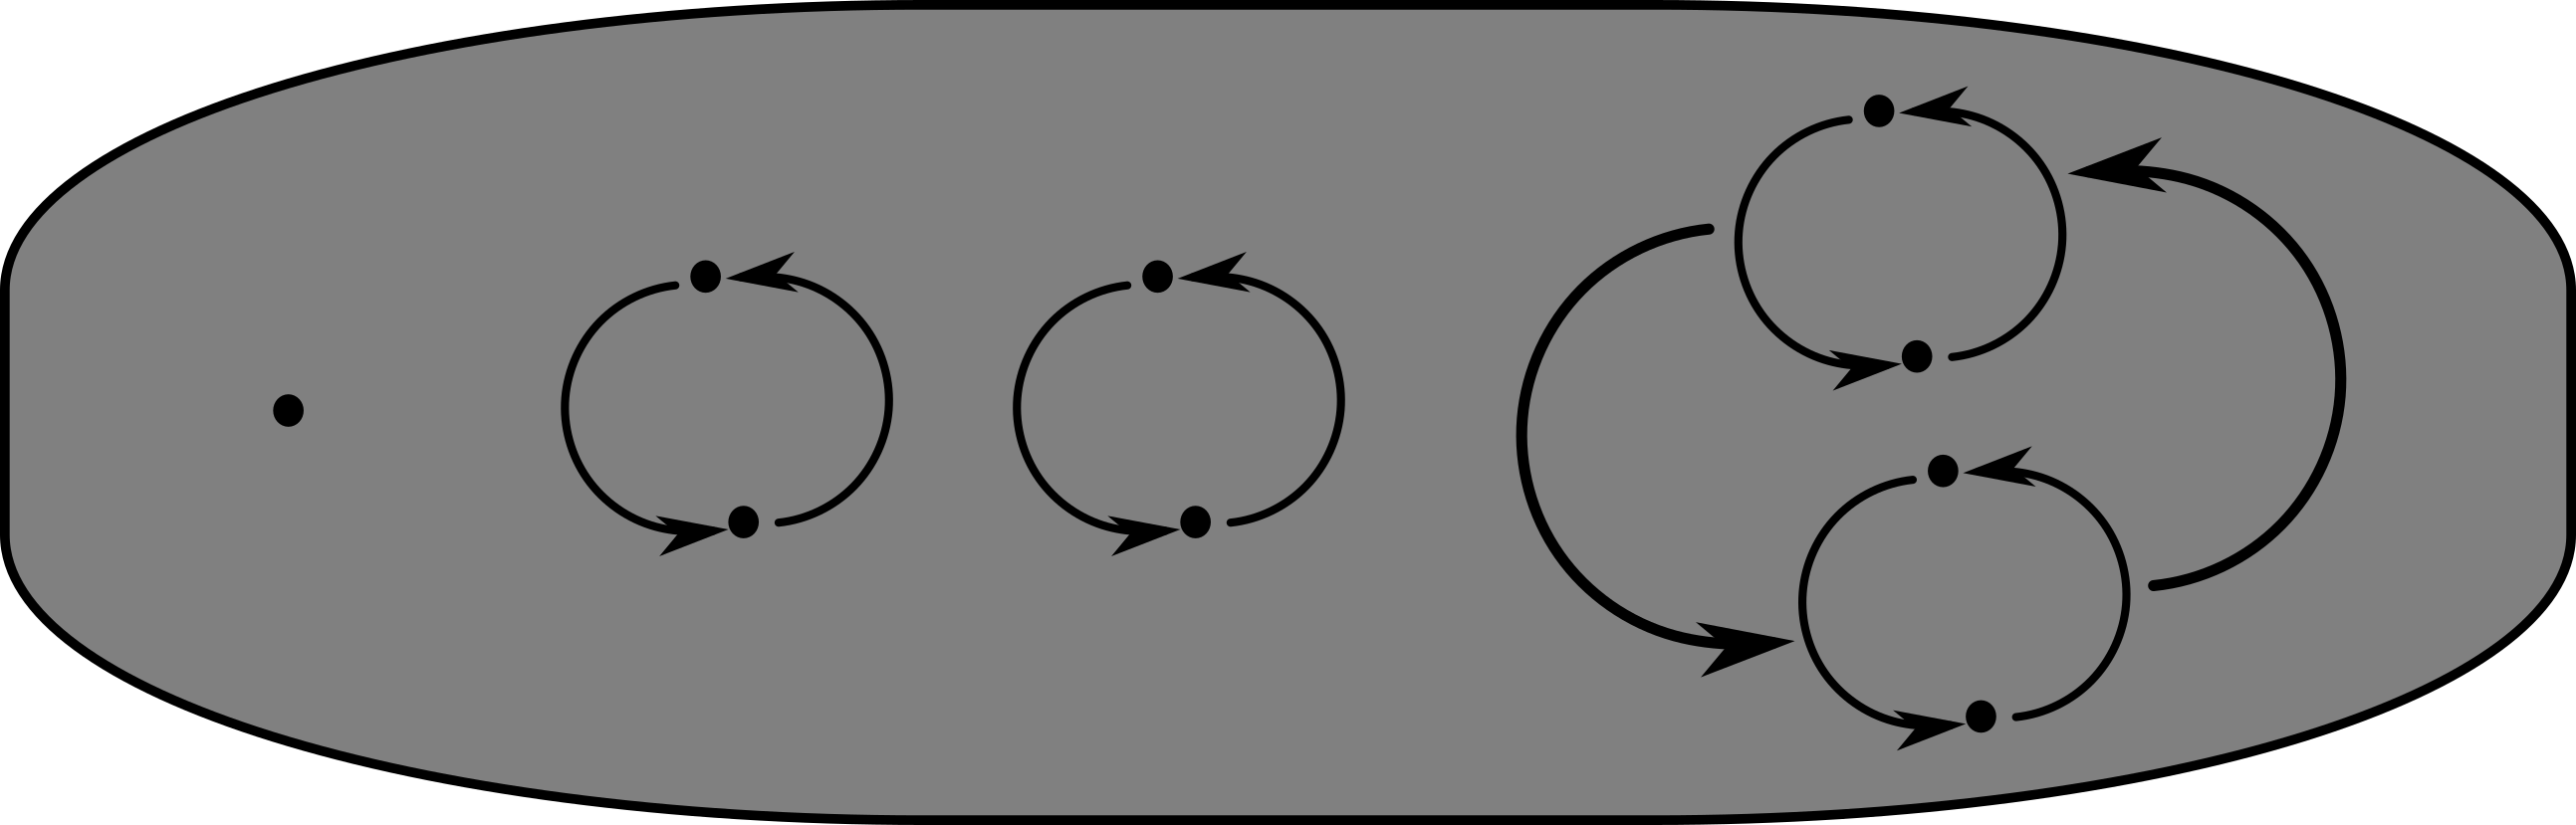
\includegraphics[scale=0.7]{figures/monomial.png}
 \caption{The class in $H_5(C_9(\D))$ corresponding to the monomial $\epsilon\cdot(Q\epsilon)^2\cdot Q^2\epsilon$.}
\label{fig:monomial}
\end{figure}

In this article we will only need the isomorphism in equation \ref{eq:Cohen} to hold as
an isomorphism of bigraded $\Z_2-$vector spaces.
In particular for all choices of natural numbers $(\alpha_j)_{j\geq 0}$ with all but finitely
many $\alpha_j=0$, we will consider the monomial $\prod_j\pa{Q^j\epsilon}^{\alpha_j}$, corresponding to
a homology class in some bidegree $(*,m)$: all that
we are going to need is that the set of these monomials is a bigraded basis for the
left-hand side of equation \ref{eq:Cohen}.

\section{Homology of configuration spaces of surfaces}
\label{sec:HBraidSurf}
We want to understand the homology groups $H_*(\bms)=H_*(C_m(\sg))$: we
are interested in these groups as they appear as the homology of the fiber
in the Leray-Serre spectral sequence associated to
\ref{eq:Birman}, \ref{eq:Birmanbundle} or \ref{eq:BirmanbundleD}.
In particular we are interested in $H_*(C_m(\S))$
as a $\Z_2-$representation of the group $\gg$.

In \cite{LM} L\"offler and Milgram proved that this must be a $\Z_2-$symplectic
representation of the mapping class group. By \emph{$\Z_2-$symplectic} we mean the following:
\begin{defn}
 \label{defn:symplrep}
 Let $\H=H_1(\S)\simeq\Z_2^{2g}$.
 The natural action of $\gg$ on $\H$ induces a surjective map
 $\gg\to Sp_{2g}(\Z_2)$. A representation of $\gg$ over $\Z_2$ is called \emph{$\Z_2-$symplectic}
 if it is a pull-back of a representation of $Sp_{2g}(\Z_2)$ along this map.
\end{defn}

In \cite{BCT} B\"odigheimer, Cohen and Taylor computed $H_*(C_m(\sg))$ \emph{as a graded $\Z_2-$vector space}.
Their method provides all Betti numbers, but the action of $\gg$ cannot be easily deduced, as
their descripition of $H_*(C_m(\sg))$ depends on a handle decomposition of $\sg$, which is not preserved,
not even up to isotopy, by diffeomorphisms of $\sg$.

In this section and in the next one we will prove the following theorem; to the best of the author's knowledge
it doesn't appear in the literature.
\begin{thm}
 \label{thm:Hbms*as*ggrep}
 There is an isomorphism of bigraded $\Z_2-$representations of $\gg$
 \[
  \bigoplus_{m\geq 0} H_*\pa{C_m(\sg)}\simeq \Z_2\left[Q^j\epsilon\,|\, j\geq 0\right]\otimes\Sym_{\bullet}(\H).
 \]
 Here we mean the following:
 \begin{itemize}
  \item the bidegree is given on left by homological degree $*$ and by the direct summand,
  indexed by $m$,
  on which the homology class is supported, i.e. by the number $m$ of points
  involved in constructing the homology class; we call $*$ the \emph{degree} and $m$ the \emph{weight},
  and write $(*,m)$ for the bidegree;
  \item for $j\geq 0$, $Q^j\epsilon$ is the image in $H_{2^j-1}(C_{2^j}(\sg))$ of a generator
  of the group $H_{2^j-1}(C_{2^j}(\D))\simeq \Z_2$ 
  under the natural map induced by the embedding $\D\hookrightarrow\mrS$,
  and $\Z_2\left[Q^j\epsilon\,|\, j\geq 0\right]$ is the polynomial ring on
  infinitely many variables $\epsilon,Q\epsilon,Q^2\epsilon,\dots$;
  \item $\H=H_1(\sg)$ is identified with $H_1(C_1(\S))$ in a natural way, and $\Sym_{\bullet}(\H)$ is the
  symmetric algebra on $\H$;
  %\item degrees and weights are extended on right by the usual multiplicativity-additivity rule;
  \item the action of $\gg$ on right is the diagonal action on the product: it is a trivial action
  on the factor $\Z_2[Q^j\epsilon\,|\, j\geq 0]$ and it is the $\Z_2-$symplectic action on the
  factor $\Sym_{\bullet}(\H)$ induced by the $\Z_2-$symplectic action on $\H$.
  \end{itemize}
\end{thm}
Notice that for any bi-homogeneus element in the right-hand side, the weight is greater or equal than
the degree: indeed factors of the form $Q^j\epsilon$ have weight strictly higher than the degree,
whereas factors in $\H$ and its symmetric powers have equal weight and degree.
  
Notice that in the case $g=0$ the group $\Gamma_{0,1}$ is trivial and the previous theorem
reduces to equation \ref{eq:Cohen}.
% isomorphism of bigraded vector spaces
% \begin{equation}
% \label{eq:genuszero}
% \bigoplus_{m\geq 0} H_*\pa{C_m(\Sigma_{0,1})}\simeq \Z_2[Q^j\epsilon\,|\, j\geq 0].
% \end{equation}
% This isomorphism was essentially proved by Fuchs in \ref{Fuchs:CohomBraidModtwo}. Moreover the left hand
% side is the homology of the space $\coprod_{m\geq 0} C_m(\Sigma_{0,1})$, which has a natural structure
% of algebra over the operad $E^2$ of little $2-$cubes. The isomorphism in equation \ref{eq:genuszero}
% is an isomorphism of rings (using the Pontryagin product on the left hand side), and $Q$ represents here
% the Araki-Kudo-Dyer-Lashof operation $Q\colon H_*(X;\Z_2)\to H_{2*+1;\Z_2}(X)$,
% which is defined for any $E^2-$algebra $X$; $\epsilon\in H_0(C_1(\Sigma_{0,1}))$ is the generator.
% This explains our notation; we refer to Cohen \cite[Chap.3]{CLM} for more details.

In this section we will prove that there is an isomorphism of \emph{bigraded $\Z_2-$vector spaces}
as in theorem \ref{thm:Hbms*as*ggrep}; in the next section we will deal with the action of
$\gg$.
%In these two sections we abbreviate $\S=\sg$.

Since we work with coefficients in the field $\Z_2$, it is equivalent to compute homology or cohomology,
and in this section we will prefer to compute $H^*(\cms)$ for all bidegrees $(*,m)$.
% the dual graded vector space $H_*(\cms)$ is abstractly isomorphic,
% i.e. it has the same dimension.

We will mimic the method used by Fuchs (\cite{Fuchs:CohomBraidModtwo}) to compute the $\Z_2-$cohomology
of $C_m(\D)$.
As already said this computation recovers a known result, but it has the advantage of
being quite elementary and of providing a part of
the geometric insight that we will need in the next section.

In the whole section we assume $m\geq 0$ to be fixed.

We first introduce a space $\T(\S)$ which is homeomorphic to $\mrS$, the interior of $\S$. The construction
corresponds to a handle decomposition of $\S$ with one $0-$handle and $2g$ $1-$handles.

\begin{defn}
\label{defn:Tsg}
If $g=0$, hence $\S=\sg$ is the disc, we set $\T(\S)=(0,1)^2$, the interior of the unit square. Assume
now $g\geq 1$.

Dissect the interval $[0,1]$ into $2g$ equal subintervals through the points $\cP_i=\frac{i}{2g}$ for $0\leq i\leq 2g$
(for $i=0,2g$ we get the two endpoints of $[0,1]$).

Let $Q\subset[0,1]^2$ be the union of $(0,1)^2$ and the vertical open intervals
$I_i^l=\set{0}\times (\cP_i,\cP_{i+1})$ and $I_i^r=\set{1}\times (\cP_i,\cP_{i+1})$ for $1\leq i\leq 2g$;
equivalently, we remove from $[0,1]^2$ the two horizontal sides
$[0,1]\times\set{0,1}$ and the $4g-2$ points $\set{0,1}\times \set{\cP_1,\dots,\cP_{2g-1}}$.

Notice that all intervals $I_i^l$ and $I_j^r$ are
canonically diffeomorphic
to $(0,1)$ by projecting on the second coordinate, rescaling linearly by a factor $2g$
and translating; therefore we will specify a bijection
between the two sets of left and right intervals, and then $\T(\S)$ will be obtained from $Q$
by identifying in the canonical way the two intervals in each couple.

For $1\leq i\leq g$, we identify $I^l_{2i-1}$ with $I^r_{2i}$, obtaining an open interval $\U_i\subset\T(\S)$,
and we identify $I^r_{2i-1}$ with $I^l_{2i}$, obtaining an open interval $\V_i\subset\T(\S)$.
Each interval $\U_i,\V_i$ has a natural parametrisation by $(0,1)$.

The space $\T(\S)$ is homeomorphic to $\mrS$. From now
on we will identify the two open surfaces and in particular we will identify $\cms$ with the
space of configurations of $m$ points in $\T(\S)$.

Let $\D\subset\mrS$ be the open square $(1/4;3/4)\times(1/2,1)$:
$\D$ is an open disc in $\mrS$ near $\partial\S$ and 
it is disjoint from all $\U_i$'s and $\V_i$'s.
\end{defn}

In the following we will consider the one-point compactification of some spaces that
happen to be open manifolds. For a space $\mathcal{M}$ we denote by $\mathcal{M}^c$ its one-point
compactification; the basepoint is the point at infinity, that we always denote by $\infty$, even
if it is a different point for different spaces $\mathcal{M}^c$.

We consider in particular the one-point-compactification $\cms^c$ of $\cms$.
Since the space $\cms$ is homeomorphic to the interior of a compact
$2m-$manifold with boundary, by Poincaré-Lefschetz
duality we have
\[
 H^*(\cms)\simeq \tilde H_{2m-*}(\cms^c).
\]
Our next aim is to define a cell structure on the space $\cms^c$.
\begin{defn}
\label{defn:ehopen}
A \emph{tuple} $\tup$ is a choice of the following set of data:
 \begin{itemize}
  \item a natural number $0\leq l\leq m$;
  \item integers $x_1,\dots,x_l\geq 1$;
  \item integers $u_1,\dots,u_g$ and $v_1,\dots,v_g$, all $\geq 0$.
 \end{itemize}
with the condition that
\[
 m=\sum_{i=1}^lx_i+\sum_{i=1}^g(u_i+v_i).
\]
% We will generically use the letter $m$ to denote any of the numbers $l$, $x_i$,$y_i$,$z$,$u_i$,$v_i$ or $w_i$
% in the above sum, so $m\in\Z$; instead .
% Similarly we will use the letter $\M$ to denote any of the intervals $\U_i,\V_i,\W_i$;
% they will correspond to the letters $U_i,V_i,W_i$, so we also define a subset
% $\bsymb=\set{(U_i,V_i)_{i\leq g},(W_i)_{i\leq n-1}}\subset\symb$.

The \emph{degree} of $\tup$ is defined as $m+l$.

For a tuple $\tup$ let $e^{\tup}$ be the subspace
of $\cms$ of configurations of $m$ points in $\mrS$ such that
\begin{itemize}
 \item for all $1\leq i\leq g$, exactly $u_i$ points lie on $\U_i$
 and exactly $v_i$ points lie on $\V_i$;
 \item there are exactly $l$ vertical lines in $(0,1)^2\subset\mrS$ of the
 form $\set{s_i}\times(0,1)$ for some $0<s_1<\dots<s_l<1$, containing at least one
 point of the configuration. From left to right, these lines contain exactly $x_1,\dots,x_l$ points
 respectively.
\end{itemize}
\end{defn}
The space $e^{\tup}$ is homeomorphic to \emph{the interior} of the following product of simplices:

% We want to show that the collection of the $e_h$ for varying $h$, together with
% the 0-cell $*$, give a cell decomposition of $C_k(\S)^c$. Denote by $\Delta^h$ the following product of simplices
\[
 \Delta^{\tup}\colon =
 \Delta^l\times\prod_{i=1}^l\Delta^{x_i}\times\prod_{i=1}^g\pa{\Delta^{u_i}\times\Delta^{v_i}},
%  =\prod_{m\in\symb_l}\Delta^m.
\]
where the simplex $\Delta^r$ is the subspace of $[0,1]^r$ of sequences $0\leq \tau_1\leq\dots\leq\tau_r\leq 1$
(the numbers $\tau_1,\dots,\tau_r$ are the \emph{local coordinates} of the simplex). The homeomorphism is given
as follows:
\begin{itemize}
 \item the local coordinates of the $\Delta^l-$factor correspond to the positions $s_1,\dots,s_l$ of the vertical
 lines in $(0,1)^2$ containing points of the configuration;
 \item the local coordinates of the $\Delta^{x_i}-$factor correspond to the positions of the $x_i$ points
 lying on the vertical line $\set{s_i}\times(0,1)$;
 \item the local coordinates of the $\Delta^{u_i}-$factor correspond to the positions of the $u_i$ points
 lying on $\U_i$, which is canonically identified with $(0,1)$; similarly for the $\Delta^{v_i}-$factor,
 with $v_i$ and $\V_i$ instead of $u_i$ and $\U_i$.
\end{itemize}
Notice that the dimension of $\Delta^{\tup}$ is equal to the degree of $\tup$.
The embedding $\mathring{\Delta}^{\tup}\cong e^{\tup}\hookrightarrow \cms^c$ extends to a continuous map
$\phi^{\tup}\colon\Delta^{\tup}\to\cms^c$, so that the image of $\partial\Delta^{\tup}$ is contained in the union of
all subspaces $e^{\tup'}$ for tuples $\tup'$ with \emph{lower} degree than $\tup$, together with the point $\infty$.

The construction of the map $\phi^{\tup}$ is as follows:
\begin{enumerate}
\item we identify the one-point compactification
$(\mrS)^c$ of $\mrS=\T(\S)$ as the quotient of $[0,1]^2$ that identifies left and right intervals as in
in definition \ref{defn:Tsg} of $\T(\S)$, and moreover collapses $[0,1]^2\setminus Q$ to the point $\infty$;
\item we consider the $m-$fold symmetric product $\SP^m\pa{(\mrS)^c}$: it contains 
as an \emph{open} subspace $\cms$, so we can identify $\cms^c$ as the quotient of $\SP^m\pa{(\mrS)^c}$ collapsing
the subspace $\SP^m\pa{(\mrS)^c}\setminus\cms$ to $\infty$;
\item the homeomorphism $\mathring{\Delta}^{\tup}\to e^{\tup}\subset\cms$ extends
now to a map $\Delta^{\tup}\to\SP^m\pa{[0,1]^2}$, that we can then further project to
$ \SP^m\pa{(\mrS)^c}$ and then to $\cms^c$: the composition
is the map $\phi^{\tup}$.
\end{enumerate}

Therefore the collection of the $e^{\tup}$, together with the $0-$cell given by $\infty$,
give a cell decomposition of $\cms^c$, with characteristic maps of cells $\phi^{\tup}$.

We can easily use these characteristic maps to compute the \emph{reduced} cellular chain complex of $\cms^c$
with coefficients in $\Z_2$, which
reads as follows.
\begin{lem}
\label{lem:doperatoropenmodtwo}
Let $\tup=(l,(x_i)_{i\leq l},(u_i,v_i)_{i\leq g})$ and
$\tup'=(l-1,(x'_i)_{i\leq l-1},(u'_i,v'_i)_{i\leq g})$
be tuples in consecutive degrees $m+l$ and $m+l-1$, and let $[\partial \tup\colon\tup']\in\Z_2$ denote the coefficient
of $\tup'$ in $\partial \tup$ in the reduced chain complex $\tilde\Ch_*(\cms^c)$.
Then $[\partial \tup:\tup']=0$ unless one (and exactly one) of the following situations occur:
\begin{itemize}
 \item $l\geq 2$ and $\tup'$ is obtained from $\tup$ by decreasing $l$ by 1, setting $x'_i=x_i+x_{i+1}$
 for one value $1\leq i\leq l-1$, and shifting the values
 $x'_j=x_{j+1}$ for $i+1\leq j\leq l-1$. We call this way to obtain $\tup'$ from $\tup$ an \emph{inner differential}.
 In this case
 \[
  [\partial \tup\colon\tup']=\binom{x_i+x_{i+1}}{x_i}.
 \]
 This binomial coefficient may be anyway equal to $0\in\Z_2$.
 \item $l\geq 1$ and $\tup'$ is obtained from $\tup$ by decreasing $l$ by 1, choosing a splitting of $x_1$
 in integers $\delta u_i,\delta v_i\geq 0$
 \[
  x_1=\sum_{i=1}^g \pa{\delta u_i+\delta v_i},
 \]
 setting $u'_i=u_i+\delta u_i$ and $v'_i=v_i+\delta v_i$ for all $1\leq i\leq g$ and shifting the values
 $x'_j=x_{j+1}$ for $1\leq j\leq l-1$. We call this a \emph{left, outer differential}. In this case
 \[
  [\partial \tup\colon\tup']=\prod_{i=1}^g\binom{u_i+\delta u_i}{u_i}\binom{v_i+\delta v_i}{v_i}.
 \]
 This binomial coefficient may be anyway equal to $0\in\Z_2$.
 \item $l\geq 1$ and $\tup'$ is obtained from $\tup$ by decreasing $l$ by 1, choosing a splitting of $x_l$
 in integers $\delta u_i,\delta v_i\geq 0$
 \[
  x_l=\sum_{i=1}^g \pa{\delta u_i+\delta v_i},
 \]
 setting $u'_i=u_i+\delta u_i$ and $v'_i=v_i+\delta v_i$ for all $1\leq i\leq g$ and keeping $x'_i=x_i$ for all $1\leq i\leq l-1$.
 We call this a \emph{right, outer differential}. Also in this case
 \[
  [\partial \tup\colon\tup']=\prod_{i=1}^g\binom{u_i+\delta u_i}{u_i}\binom{v_i+\delta v_i}{v_i}.
 \]
 This binomial coefficient may be anyway equal to $0\in\Z_2$.
\end{itemize}
\end{lem}
\begin{proof}
 If we restrict the map $\phi^{\tup}\colon\Delta^{\tup}\to\cms^c$ to any face of the multisimplex
 $\Delta^{\tup}$ coming from a factor different from $\Delta^l$,
 we obtain a constant map to $\infty$, hence these faces don't contribute
 to the boundary of $e^{\tup}$ in the reduced cellular chain complex. Instead for $0\leq i\leq l$ the restriction
 \[
  \phi^{\tup}\colon\partial_i\Delta^l\times\prod_{i=1}^l\Delta^{x_i}\times\prod_{i=1}^g\pa{\Delta^{u_i}\times\Delta^{v_i}}\to\cms^c
 \]
 hits homeomorphically the open cell $e^{\tup'}$
 exactly as many times as specified in the statement
 of the lemma for the cases $1\leq i\leq l-1$,
 $i=0$ and $i=l$ respectively, and no other open cell.
 We are working in $\Z_2$ so we don't have to be careful about orientations of simplices
 and therefore about signs.
\end{proof}

We can filter the chain complex $\tilde\Ch_*(\cms^c)$ by giving norm $\sum_{i=1}^lx_i$ to
the cell $e^{\tup}$, with $\tup=(l,(x_i)_{i\leq l},(u_i,v_i)_{i\leq g})$. By lemma \ref{lem:doperatoropenmodtwo}
the norm is weakly decreasing along boundaries. Let $F_p\subset\tCh_*(\cms^c)$ be the subcomplex of cells
of norm $\leq p$, and let $F_p/F_{p-1}$ be the $p-$th filtration stratum.

Then $F_p/F_{p-1}$ is isomorphic, as a chain complex, to a direct sum of copies of $\tCh_*(C_p(\Sigma_{0,1}))$,
one copy for each way of splitting $m-p=\sum_{i=1}^g (u_i+v_i)$ with $u_i,v_i\geq 0$; the isomorphism
doesn't preserve the degrees but shifts them by $p$.

Indeed in $F_p/F_{p-1}$ all outer
differentials vanish (see lemma \ref{lem:doperatoropenmodtwo}
for the definition), in particular the numbers $u_i,v_i$
don't change along the boundary map of $F_p/F_{p-1}$, and this latter chain complex splits as a direct sum
of chain complexes indexed by splittings $m-p=\sum_{i=1}^g (u_i+v_i)$ as above.
It is then immediate to identify the inner differentials
with the ones one would have in the case $g=0$, i.e. for the surface $\Sigma_{0,1}$.

We notice that $\tCh_*(C_p(\Sigma_{0,1})^c)$ is exactly the chain complex described by Fuchs in
\cite{Fuchs:CohomBraidModtwo}, so we pause for a moment and
recall some classical facts about the cohomology of configuration
spaces of the disc.
\begin{defn}
\label{defn:symchain}
Given a splitting $p=\sum_{j=0}^{\infty}\alpha_j2^j$ of $p$ into powers of 2, with multiplicities $\alpha_j$,
the associated symmetric chain in $\tCh_*(C_p(\Sigma_{0,1})^c)$
is the sum of all $e^{\tup}$ where $\tup$ ranges among all tuples
$\pa{l,(x_i)_{i\leq l}}$ such that
\begin{itemize}
 \item $l=\sum_{j=1}^{\infty}\alpha_j$;
 \item every $x_i$ is a power of 2;
 \item for all $j\geq 0$ there are exactly $\alpha_j$ indices $i$ such that $x_i=2^j$.
\end{itemize}
Here and in the following it is understood that $\alpha_j=0$ for all but finitely many indices $j$.

We denote by $|(\alpha_j)_{j\geq 0}|\in\tCh_{p+l}(C_p(\Sigma_{0,1})^c)$ the symmetric chain
and by $[(\alpha_j)_{j\geq 0}]\in\tH_{p+l}(C_p(\Sigma_{0,1})^c)$ the associated homology class.
\end{defn}
In \cite{Fuchs:CohomBraidModtwo} Fuchs shows that a graded basis for $\tH_*(C_p(\Sigma_{0,1})^c)$
is given by the collection of all classes $[(\alpha_j)_{j\geq 0}]$ satisfying $\sum\alpha_j2^j$.

Using Poincaré-Lefschetz duality we obtain a basis for the cohomology of $C_p(\Sigma_{0,1})$;
the dual basis of $H_*(C_p(\Sigma_{0,1}))$
happens to be the basis of monomials
$\prod_{j\geq 0}(Q^i\epsilon)^{\alpha_j}\in H_*(C_p(\Sigma_{0,1}))$ of weight $m$, using
the isomorphism \ref{eq:Cohen} in its full meaning (i.e. as an isomorphism of rings,
where $Q$ denotes the first Dyer-Lashof operation).

% This notation is compatible, after interpreting equation \ref{eq:genuszero} as an isomorphism
% of rings, with the results of \cite[Chap.3]{CLM}: the monomials constructed there, using
% the Pontryagin product and the operation $Q$, are really the dual basis of the basis of
% symmetric chains for cohomology.

We will not need this finer result in this article, so the expression
$\prod_{j\geq 0}(Q^i\epsilon)^{\alpha_j}\in H_{p-l}(C_p(\Sigma_{0,1}))$ will only denote
the (unique) homology class whose algebraic intersection with $[(\alpha'_j)]\in\tH_{p+l}(C_p(\Sigma_{0,1})^c)$
is $1\in\Z_2$ if and only if the equality $\alpha_j=\alpha'_j$ holds for all $j\geq 0$.
% i.e. we \emph{define} monomials as the dual basis of the basis of symmetric chains, and keep considering
% \ref{eq:Cohen} only as an isomorphism of bigraded vector spaces.

We now go back to the filtered chain complex $\tCh_*(\cms^c)$:
if we run the associated Leray spectral sequence,
the $E^1-$page contains on the $p-$th column the homology of $F_p/F_{p-1}$; as we have seen this consists of
many copies of the homology of $\tCh_*(C_p(\Sigma_{0,1}))$, each generated by symmetric chains.

\begin{defn}
\label{defn:gensymchain}
For a splitting
\[
 m=p+(m-p)=\pa{\sum_{j=0}^{\infty}\alpha_j2^j}+\pa{\sum_{i=1}^g(u_i+v_i)}
\]
we define a chain in $\tCh_{m+l}(\cms)$, denoted by $|p,(\alpha_j)_j,(u_i,v_i)_{i\leq g}|$: it
is obtained by summing all $e^{\tup}$ where $\tup$
ranges among all tuples of the form $\pa{l,(x_i)_{i\leq l},(u_i,v_i)_{i\leq g}}$
satisfying the three properties listed in definition \ref{defn:symchain}.

We call such a chain a
\emph{generalised symmetric chain}, and its homology class in $\tH_{m+l}(\cms^c)$ is denoted
by $[p,(\alpha_j),(u_i,v_i)]$
\end{defn}

It is straightforward to check that a generalised symmetric chain $|p,(\alpha_j),(u_i,v_i)|$
is not only
a cycle when projected to its filtration quotient $F_p/F_{p-1}$, as the $E^1-$page
of the spectral sequence tells us, but also
in the chain complex $\tCh_*(\cms^c)$ itself. Indeed also all outer
differentials of a generalised symmetric chain cancel out, since
every left differential
of one cell $e^{\tup}$ in the generalised symmetric chain cancels out with a right differential
of possibly another cell $e^{\tup'}$.

In particular the spectral sequence collapses on its first page and
% $H_*(\cms^c)$
% has a $\Z_2$-basis given by generalised symmetric chains.
we have the following lemma:
\begin{lem}
\label{lem:gensymchain}
The homology $H_*(\cms^c)$ has a graded basis given by the classes $[p,(\alpha_j),(u_i,v_i)]$
associated to generalised symmetric chains.
% this basis is bijection with
% the choices of the following set of data:
% \begin{itemize}
%  \item a number $0\leq p\leq m$;
%  \item a splitting $m-p=\sum_{i=1}^g (u_i+v_i)$ with $u_i,v_i\geq 0$;
%  \item a splitting $p=\sum_{j=0}^{\infty}\alpha_j2^j$ with $\alpha_j\geq 0$.
% \end{itemize}
% The homology class $[p,(u_i,v_i),(\alpha_j)]\in H_*(\cms^c)$ has homological degree
% $m+\sum_{j=1}^{\infty}\alpha_j$.
\end{lem}
% To interpret this class
% as a monomial in the tensor product of theorem \ref{thm:Hbms*as*ggrep} we need the following definition.

% We are almost ready to prove an isomorphism of bigraded $\Z_2-$vector spaces as in theorem \ref{thm:Hbms*as*ggrep}.

\begin{defn}
 \label{defn:dualHbasis}
We can see the $\U_i$'s and $\V_i$'s as properly embedaded $1-$manifolds in $\mrS$;
by Poincaré-Lefschetz duality they represent classes in $H_1\pa{(\mrS)^c}\simeq H^1(\S)$,
and in particular they form a basis
of the latter cohomology group. We call $\u_i,\v_i\in H_1\pa{\mrS}$ the dual basis.

% We fix simple closed curves $\u_i,\v_i$ on $\S$, for $1\leq i\leq g$, whose fundamental classes
% $[\u_i],[\v_i]$ form the dual basis of $H_1(\S)$. We assume that, apart from the following necessary exceptions,
% all curves $\U_i,\V_i,\u_i,\v_i$ for $1\leq i\leq g$ are disjoint:
% \begin{itemize}
%  \item $\u_i$ and $\v_i$ intersect once, transversely;
%  \item $\u_i$ and $\U_i$ intersect once, transversely;
%  \item $\v_i$ and $\V_i$ intersect once, transversely;
%  \end{itemize}
% SEE PICTURE.
\end{defn}
We establish a bijection between monomials in the tensor product of theorem  \ref{thm:Hbms*as*ggrep}
and the basis of $H^*(\cms)\simeq H_*(\cms^c)$ in lemma \ref{lem:gensymchain}:
the class 
\[
[p,(u_i,v_i),(\alpha_j)]\in H_{m+\sum\alpha_j}(\cms^c)\simeq H^{m-\sum\alpha_j}(\cms)
\]
is associated with the monomial $\prod_{j=1}^{\infty}(Q^j\epsilon)^{\alpha_j}\otimes \prod_{i=1}^g([\u_i]^{u_i}[\v_i]^{v_i})$.

This shows an isomorphism of bigraded $\Z_2-$vector spaces
\begin{equation}\label{eq:isovectorspaces}
  \bigoplus_{m\geq 0} H^*(\cms)\simeq \Z_2\left[Q^i\epsilon\,|\, i\geq 0\right]\otimes\Sym_{\bullet}(\H),
\end{equation}

and using the canonical identification of $\Z_2-$cohomology as the dual of homology, we can
conclude that there exists an isomorphism as in theorem \ref{thm:Hbms*as*ggrep}
at least \emph{as bigraded $\Z_2-$vector spaces}.



\section{Action of $\gg$}
\label{sec:Actiongg}
We now turn back to \emph{homology} of $\cms$. In the first subsection we describe geometrically some
homology classes, in order to give some intuition for the following subsections.
In the second subsection we prove Theorem
\ref{thm:Hbms*as*ggrep} in bigradings $(*,m)$ with $*=m$.
In the third subsection we extend the proof to all other bigradings.

\subsection{Geometric examples of homology classes}
In this subsection we consider the surface $\Sigma_{2,1}$, which we abbreviate with $\S$, and
construct some homology classes in $H_2(C_2(\S))$: our aim is to get a first understanding
of why this homology group is isomorphic to $\Sym_2(\H)=\H^{\otimes 2}/\mathfrak{S}_2$.


\subsection{Bigradings of the form $(m,m)$}
In this subsection we construct a $\gg$-~equivariant isomorphism 
\[
\psi_m\colon \Sym_m(\H))\to H_m(\cms).
\]
% the former group is isomorphic to $\Sym_m(H^1(\S))$ and the second to $H^m(\cms)$,
% both by Poincaré-Lefschetz duality.

We already know that these $\Z_2$-vector spaces have the same dimension:
indeed $\Sym_m(\H)$ is precisely the summand in bigrading $(m,m)$ in equation
\eqref{eq:isovectorspaces}, using that a monomial
 whose
weight is \emph{equal} and not bigger than its degree cannot contain factors of the form
$Q^i\epsilon$.
% i.e. it must lie in the factor $\Sym_{\bullet}(\H)$, and if the degree
% is $m$ it must lie in $\Sym_m(\H)$.
% 
% The rough idea in constructing the map $\psi_m$ is the following: $\Sym_m(\H)$ is generated
% by elements of the form $[c_1]\cdot\ldots\cdot[c_m]$, where $c_1,\dots,c_m\colon\Sone\to\mrS$ are simple
% closed curves; we consider the product map 
% \[
% c_1\times\dots\times c_m\colon \pa{\Sone}^{\times m}\to \SP^m(\mrS)
% \]
% which carries the fundamental class of the $m$-fold torus to some class in
% $H_m(\SP^m(\mrS))$; we then lifts this class, in a nice way, to a class
% in $H_m(\cms)$.


The construction of $\psi_m$ is rather long and technical and involves a few definitions.

\begin{defn}
\label{defn:DinTS} 
Recall Definition \ref{defn:TS}. We denote by $\D\subset\T(\S)\cong\mrS$ the open square $]1/4;3/4[\times]1/2,1[$.
Note that $\D$ is an open disc in $\mrS$ near $\partial\S$ and 
it is disjoint from all $\overline{\U}_i$'s and $\overline{\V}_i$'s. The interior of the surface $\S'$
is then identified with $\T(\S)\setminus [1/4,3/4]\times[1/2,1[$.
\end{defn}


\begin{defn}
\label{defn:cCm}
Let $\cC^m$ be the the (discrete) set of isotopy classes of $m$-tuples of simple closed curves $c_1,\dots,c_m\subset\mrS$
such that
%\begin{itemize}
%  \item each $c_r\colon\Sone\to\mrS$ is smooth and transverse to each $\U_i$ and $\V_i$;
% \item
 any two curves $c_i,c_j$ intersect each other only inside $\D$.
 
% \item each curve $c_i$ is transverse to $\partial\D$.
%\end{itemize}
Curves are seen as maps $\Sone\to\mrS$, and the intersection of two curves is the intersection of their
images. Here and in the following $\Sone$ is the unit circle in $\C$.

Two $m$-tuples of curves are isotopic if there is an ambient isotopy of $\S$ relative to $\partial\S\cup\D$
transforming one $m$-tuple into the other. In particular $\cC^m$ is more than countable.

An element of $\cC^m$ is called \emph{multicurve}; by abuse of notation the $m$-tuple
$(c_1,\dots,c_m)$ will often represent its class in $\cC^m$, i.e. the corresponding multicurve.
See picture \ref{fig:defcCm}
% For each isotopy class we
% suppose to have fixed a representative $(c_1,\dots,c_m)$ made of curves that are
% also transverse to all $\U_i$'s and $\V_i$'s. We write
% $[c_1,\dots,c_m]$ for the isotopy class whose preferred representative is
% $(c_1,\dots,c_m)$.

We denote by $\ZcC{m}$ the free $\Z_2$-vector space with basis $\cC^m$.
There is a canonical surjective map $\pr_m\colon\ZcC{m}\to\Sym_m(\H)$ given by
\[
 \pr_m(c_1,\dots,c_m)=[c_1]\cdot\ldots\cdot[c_m],
\]
where $[c_i]\in\H$ is the fundamental class of the curve $c_i$.

The group $\gg$ acts both on $\ZcC{m}$, by acting on its basis $\cC^m$, and
on $\Sym_m(\H)$, symplectically. The map $\pr_m$ is $\gg$-equivariant.
\end{defn}

\begin{figure}\centering
 \includegraphics[scale=0.7]{figures/defcCm.pdf}
 \caption{A multicurve in $\cC^5$.}
\label{fig:defcCm}
\end{figure}

% Our aim is to define a $\gg$-equivariant map $\tpsi\colon\ZcC{m}\to H_m(\cms)$ and show that it
% factors through $\pr$ to give the desired $\gg$-equivariant map $\psi$; we will then show that
% $\psi$ is an isomorphism.

% The map $\tpsi_m$ that we construct will have two additional properties. The first
% is the following: for any
% $(c_1,\dots,c_m)$ representing a class in $\cC^m$, the homology
% class $\tpsi_m(c_1,\dots,c_m)$ can be represented by a singular cycle in $\cms$ which
% is \emph{supported} on the union $\D\cup c_1\cup \dots\cup c_m$, meaning that
% this singular cycle only hits configurations in $\cms$ whose points actually
% lie in $\D\cup c_1\cup \dots\cup c_m$.
% 
% For the second property we need a definition
\begin{defn}
 \label{defn:cmsD}
 Recall Definition \ref{defn:SP}.
 The space $\cmsD$ is the subspace of $\SP^m(\mrS)$ of configurations where all points
 having multiplicity $\geq 2$ lie inside $D$.
 See Figure \ref{fig:defcmsD}.
 
  Note that $\cmsD$ is open in $\SP^m(\mrS)$. There is an open inclusion $\iota_m\colon\cms\subset\cmsD$ and there is a natural map
  \[
  \j_m\colon \ZcC{m}\to H_m(\cmsD)
  \]
  defined as follows: for a class $(c_1,\dots,c_m)\in\cC^m$
  the composition
  \[
   \begin{CD}
    \pa{\Sone}^{\times m} @>c_1\times\dots\times c_m >> (\mrS)^{\times m} @>>> \SP^m(\mrS)
   \end{CD}
  \]
has image in the subspace $\cmsD$; we define $\j_m(c_1,\dots,c_m)$ as the image
of the fundamental class
of the $m$-fold torus in $H_m(\cmsD)$. The result does not change
if we substitute $(c_1,\dots,c_m)$ with another isotopic $m$-tuple of curves in the same multicurve.

We call $[c_1]\cdot\ldots\cdot[c_m]$ the image in the singular chain complex of $\cmsD$ of
the fundamental cycle of the
$m$-fold torus: this cycle represents the class $\j_m(c_1,\dots,c_m)$ and it is \emph{supported}
on the union $c_1\cup\dots\cup c_m$, meaning that it hits configurations in $\cmsD$ of points of $\mrS$
lying in this union.

The group $\Diff(\S,\D\cup\partial\S)$ acts on $\cmsD$, and there is an induced action of $\gg$
on $H_m(\cmsD)$. The map $\j_m$ is $\gg$-equivariant.
\end{defn}

\begin{lem}
 \label{lem:cms->cmsDinj}
 The inclusion $\iota_m\colon\cms\to\cmsD$ induces an injective map
 \[
  \pa{\iota_m}_*\colon H_m(\cms)\to H_m(\cmsD).
 \]
\end{lem}
\begin{proof}
 It is equivalent to prove that the map $\iota_m^*\colon H^m(\cmsD)\to H^m(\cms)$ is surjective,
 or, using Poincaré-Lefschetz duality, that the map $\tH_m(\cmsD^{\infty})\to \tH_m(\cms^{\infty})$
 is surjective: this last map is induced by the map $\cmsD^{\infty}\to\cms^{\infty}$ collapsing the subspace
 $\cmsD^{\infty}\setminus\cms$ to $\infty$.
 
 Recall Lemma \ref{lem:gensymchain} and Definition \ref{defn:gensymchain}. A basis for $\tH_m(\cms^{\infty})$
 is given by classes $[\kappa(0,\uu,\uv)]$, with
 $\uu=(u_1,\dots, u_g)$, $\uv=(v_1,\dots,v_g)$ and
 $\sum_{i=1}^g (u_i+v_i)=m$.
 
 The class $[\kappa(\uu,\uv)]$ is represented by a generalised symmetric chain consisting of only one tuple $\tup=(0,\uu,\uv)$.
 
 In particular there is a map of pairs
 $\phi^{\tup}\colon(\Delta^{\tup},\partial\Delta^{\tup})\to (\cms^{\infty},\infty)$, and the class $[\kappa(\uu,\uv)]$
 is the image along this map of the fundamental class of $H_m\pa{\Delta^{\tup},\partial\Delta^{\tup}}$.
 
 It is straightforward to check that the map $\phi^{\tup}$ factors through
 $(\cmsD,\infty)$, as a map of pairs; surjectivity of $\tH_m(\cmsD^{\infty})\to \tH_m(\cms^{\infty})$ follows.
\end{proof}

We have the following diagram of $\gg$-equivariant maps, where the full arrows are those
that we have already constructed, and we still have to prove the existence of the dashed arrows
\begin{equation}
\label{eq:fulldasheddiagram}
\begin{tikzcd}[column sep=8em,row sep=5em]
  \ZcC{m} \ar[r,"\pr_m",two heads]\ar[d,dashed, swap, "\tpsi_m"]\ar[dr,"\j_m",near start]
  & \Sym_m(\H)\ar[d,dashed ]\ar[dl,dashed,very near start,"\psi_m"]\\
  H_m(\cms)\ar[r,swap,"\pa{\iota_m}*",hook] & H_m\pa{\cmsD}.
 \end{tikzcd}
\end{equation}

We now prove that the map $\j_m$ lifts along $(\iota_m)_*$
to a $\gg$-equivariant map $\tpsi_m$ as in the diagram.
Since $(\iota_m)_*$ is injective by Lemma \ref{lem:cms->cmsDinj}, it suffices to prove that $\j_m$
lands in the image of $(\iota_m)_*$, and this last statement does not depend on how $\gg$ acts on these groups.

We will prove by induction on $m$ the following technical lemma:

\begin{lem}
 \label{lem:tpsiwithproperties}
For each $m$-tuple of curves $(c_1,\dots,c_m)$ representing a class in $\cC^m$
and for each open neighborhood $\N\subset\mrS$ of
$\D\cup c_1\cup\dots\cup c_m$, there is a singular cycle $\fc=\tpsi_m(c_1,\dots,c_m)$
in $\cms$ with the following properties:
\begin{itemize}
 \item the cycle $\fc$ is \emph{supported} on $\N$, i.e.,
this singular cycle only hits configurations of $m$ distinct points of $\mrS$ that actually lie in $\N$;
\item $\pa{\iota_m}_*(\fc)$ represents the homology class $\j_m(c_1,\dots,c_m)\in H_m\pa{\cmsD}$;
\item the two cycles $\pa{\iota_m}_*(\fc)$ and $[c_1]\cdot\ldots\cdot[c_m]$
are connected by a homology in $\cmsD$ which is supported on $\N$ (the word
\emph{homology} denotes here a $(m+1)$-singular chain whose boundary is the difference between the two cycles).
\end{itemize}
\end{lem}

For $m=0$ both $\ZcC{0}$ and $H_0(C_0(\S))$ are
isomorphic to $\Z_2$ and there is nothing to show. For $m=1$
we have a canonical identification $H_1(C_1(\S))\simeq\H\simeq\Sym_1(\H)$, so we take $\tpsi_1=\pr_1$;
obviously for all $c_1$ representing a class in $\cC^1$, the homology class $\pr_1(c_1)\in\H$
is represented by a cycle supported on $c_1$,
and in this case the cycles $\iota_*\pa{\tpsi(c_1)}$ and $\pr_1(c_1)=\j_m(c_1)$ coincide.

Let now $m\geq 1$ and in the following fix a class $(c_1,\dots, c_{m+1})\in\cC^{m+1}$.
% and suppose that we have proved the existence of the lift $\tpsi_m\colon \ZcC{m}\to H_m(\cms)$
% with the aforementioned property.

\begin{defn}
\label{defn:variationsCm}
We introduce several variations of the notion of configuration space; see Figure \ref{fig:defcmsD}.
\begin{itemize} 
 \item The space $C_{1,m}(\S)$ is the subspace of $\mrS\times \cms$ containing all configurations
 $\pa{\bar P;\set{P_1,\dots,P_m}}$ with $\bar P\neq P_i$ for all $i$; in other words it is
 the space of configurations of $m+1$ points, one of which is \emph{white} (meaning that
 it is distinguishable from the other points), whereas the other are \emph{black} and not distinguishable
 from each other.
%  \item The space $\fmsD$ is the subspace of $\mrS\times\cmsD$ containing all configurations
%  $(q;\set{p_1,\dots,p_m})$ where either $q\in\D$ may coincide with some $p_i$ (which can appear
%  with multipliciy $\geq 1$), or $q\not\in\D$ must be distinct from all $p_i$'s.
%  Again $q$ is thewhite point
 \item The space $\fmstwoD$ is the subspace of $\mrS\times\cms$ containing all configurations
 $\pa{\bar P;\set{P_1,\dots, P_m}}$ where either $\bar P\in\D$ may coincide with \emph{exactly}
 one $P_i$, or
 $\bar P\not\in \D$ must be distinct from all $P_i$'s.
 Again $\bar P$ is called the white point.
 %We see that $C_{1,m}\subset\fmstwoD$ is an open subspace.
 \item The space $\cmstwoD$ is the subspace of $\SP^{m+1}(\mrS)$ of configurations where either all $m+1$ points
 are distinct, or there is exactly one point \emph{inside $\D$} with multiplicity $2$ and $m-1$ other points,
 somewhere in $\mrS$, with multiplicity $1$.
\end{itemize}
 \end{defn}
 
\begin{figure}\centering
 \includegraphics{figures/defcmsD.pdf}
 \caption{A configuration in each of the space introduced in Definitions \ref{defn:cmsD} and \ref{defn:variationsCm}.
 Whenever a multiplicity is not specified, it is equal to 1.}
\label{fig:defcmsD}
\end{figure}

 
We have the following inclusions:
\[
C_{1,m}(\S)\subset\fmstwoD\subset\mrS\times\cmsD\subset\mrS\times\SP^m(\mrS);
\]
\[
C_{m+1}(\S)\subset\cmstwoD\subset C_{m+1}^{\D}(\S)\subset\SP^{m+1}(\mrS).
\]
All these spaces are
manifolds of dimension $2m+2$ and all inclusions are open.

In particular there is a sequence of maps
\[
 H_{m+1}\pa{C_{m+1}(\S)}\to H_{m+1}\pa{\cmstwoD}\to H_{m+1}\pa{C_{m+1}^{\D}(\S)}
\]
and we will first lift the homology class $j_{m+1}(c_1,\dots,c_{m+1})$ to $H_m\pa{\cmstwoD}$ and
then to $H_{m+1}(C_{m+1}(\S))$, each time controlling the support of our representing
cycles and of the homologies between them.

Fix a neighborhood $\N$ of $\D\cup c_1\cup\dots\cup c_{m+1}$.

For the first lift, let $\N'=\pa{\N\setminus c_1}\cup\D$, which is an open
neighborhood of $\D\cup c_2\cup\dots\cup c_{m+1}$ in $\mrS$. By inductive hypothesis
there is a cycle $\fc=\tpsi_m(c_2,\dots,c_{m+1})$ in $\cms$ which is supported on $\N'$,
and such that $(\iota_m)_*(\fc)$ is homologous to $[c_2]\cdot\ldots\cdot[c_{m+1}]$
along a homology in $\cmsD$ supported on $\N'$ as well.

We can multiply both
cycles and the homology between them by the cycle $[c_1]$: the result are the two homologous cycles
$[c_1]\cdot \fc$ and $[c_1]\cdot\ldots\cdot[c_{m+1}]$ in $C_{m+1}^{\D}(\S)$: both cycles and the
homology between them are supported on $\N$. Note now that the
cycle $[c_1]\cdot\fc$ lives in $\cmstwoD$, so the first lift is done and we can now
deal with the second lift.

There is a natural map $\p\colon \fmstwoD\to \cmstwoD$, which converts the white point
into a black point. This map restricts to %maps $\fmstwoD\to\cmstwoD$ and 
a map $C_{1,m}(\S)\to C_{m+1}(\S)$, so that
% the latter being even a $m+1$-fold covering map;
we have a commutative diagram
 \begin{equation}\label{eq:cmstwodiagram}
  \begin{CD}
   C_{1,m}(\S) @>\subset >> \fmstwoD %@>\subset >> \fmsD
\\   @V\p VV @V\p VV %@V\p VV
\\   C_{m+1}(\S) @>\subset >> \cmstwoD %@>\subset >> C_{m+1}^D(\S)
   \end{CD}
\end{equation}

\begin{defn}
\label{defn:falsediagonals} 
Let 
\[
\Dmone=\cmstwoD\setminus C_{m+1}(\S)
\]
and similarly
\[
\Donem=\fmstwoD\setminus C_{1,m}(\S).
\]
We note that $\p$ restricts to a homeomorphism $\Donem\to\Dmone$. Moreover both $\Dmone\subset\cmstwoD$
and $\Donem\subset\fmstwoD$ are closed submanifolds of codimension $2$, and the map $\p$ restricts to
a $2$-fold ramified covering between their respective normal bundles.
\end{defn}

Diagram \eqref{eq:cmstwodiagram} induces a commutative diagram in homology
\begin{equation}
 \label{eq:fivediagram}
\minCDarrowwidth15pt
 \begin{CD}
  @. H_{m+1}\pa{\fmstwoD} @>>> H_{m+1}\pa{\fmstwoD, C_{1,m}(\S)}\\
  @. @V\p_*VV @V\p_*VV\\
  H_{m+1}\pa{ C_{m+1}(\S)} @>>> H_{m+1}\pa{\cmstwoD} @>>> H_{m+1}\pa{\cmstwoD,C_{m+1}(\S)}
 \end{CD}
\end{equation}

Recall that we want lift the homology class represented by the cycle $[c_1]\cdot\fc$
from the bottom central group to the bottom left group.

We first note that there is a lift of $[c_1]\cdot\fc$ to a cycle $[c_1]\otimes\fc$ in $\pa{\fmstwoD}$:
this is defined by declaring the point in $[c_1]\cdot\fc$ that spins around $c_1$
to be white. We then note that the right vertical map
\[
\p_*\colon H_{m+1}\pa{\fmstwoD, C_{1,m}(\S)} \to H_{m+1}\pa{\cmstwoD,C_{m+1}(\S)}
\]
can be rewritten, after using excision to tubular neighborhoods of $\Donem$ and $\Dmone$ respectively,
and the Thom isomorphism, as a map
\[
 H_{m-1}(\Donem)\to H_{m-1}(\Dmone).
\]
The latter map is multiplication by $2$, after identifying $\Dmone$ and $\Donem$ along $p$:
indeed the normal bundle of $\Donem$ is a
double covering of the normal bundle of $\Dmone$, hence the Thom class of the first disc
bundle corresponds to twice the Thom class of the second disc bundle. We are working
with coefficients in $\Z_2$, so multiplication by $2$ is the zero map.

Therefore the image of the cycle $[c_1]\otimes \fc$ along the diagonal of the square
in diagram \eqref{eq:fivediagram} is zero; hence the image of $[c_1]\cdot\fc$ in $H_{m+1}\pa{\cmstwoD,C_{m+1}(\S)}$
is zero; hence the homology class of $[c_1]\cdot\fc$ comes from $H_{m+1}(C_{m+1}(\S))$. More
precisely, there exists a cycle $\fc'$ in $C_{m+1}(\S)$ such that $\pa{\iota_{m+1}}_*(\fc')$ is homologous
to $[c_1]\cdot\fc$.

To prove Lemma \ref{lem:tpsiwithproperties} we need to find a good cycle and
a good homology, namely two that are supported on $\N$: a priori both $\fc'$ and the homology
between $\pa{\iota_{m+1}}_*(\fc')$ and $[c_1]\cdot\fc$ are only supported on $\mrS$.

This can be done by replacing, in the whole argument of the proof, the surface $\mrS$ with the surface $\N$.
We can define configuration spaces as in Definition \ref{defn:variationsCm} also for the open surface
$\N$, and we can repeat the argument considering $\N$ as the \emph{ambient surface}:
indeed we only needed a surface containing $\D$ and all curves $c_1,\dots,c_{m+1}$.

It is crucial that the action of $\gg$ is not involved in the statement of Lemma
\ref{lem:tpsiwithproperties}, as $\N\subset\S$ is not preserved, even up to isotopy,
by diffeomorphisms of $\S$.
Lemma \ref{lem:tpsiwithproperties} is proved.

We now have to prove the following lemma to conclude the proof of Theorem \ref{thm:Hbms*as*ggrep}
in bigradings $(m,m)$.
\begin{lem}
 \label{lem:tpsi->psi}
The map $\tpsi_m\colon\ZcC{m}\to H_m(\cms)$ is surjective and factors through the map $\pr_m$.
\end{lem}
\begin{proof}
The factorisation is equivalent to the inclusion $\ker\pr_m\subseteq\ker\tpsi_m$: since both
$\pr_m$ and $\tpsi_m$
are $\gg$-equivariant, also the induced map of vector spaces
\[
\Sym_m(\H)=\ZcC{m}/\ker\pr_m\to H_m(\cms)
\]
will automatically be
$\gg$-equivariant.

Recall from the proof of Lemma \ref{lem:cms->cmsDinj} that a basis for $\tH_m(\cms^{\infty})$ 
is given by the classes $[\kappa(\uu,\uv)]$, represented by generalised
symmetric chains consisting of only one tuple $\tup=(0,\uu,\uv)$, for some vectors
$\uu=(u_1,\dots,u_g)$ and $\uv=(v_1,\dots,v_g)$ satisfying $\sum_{i=1}^g(u_i+v_i)=m$.

The homology class
$[\kappa(\uu,\uv)]$ is the fundamental class
of the sphere $e^{\tup}\cup\set{\infty}\subset\cms^{\infty}$: the inclusion of this sphere in $\cms^{\infty}$
restricts to a proper embedding $e^{\tup}\subset\cms$.

By Poincaré Lefschetz duality $\tH_m(\cms^{\infty})\simeq H^m(\cms)$, and the latter is
the dual of $H_m(\cms)$.

We can therefore associate to $[\kappa(\uu,\uv)]$ a linear functional
on $H_m(\cms)$. This is the algebraic intersection product with the cell $e^{\tup}$, seen as a proper submanifold of $\cms$:
we denote it by
\[
 \cdot\cap e^{\tup}\colon H_m(\cms)\to\Z_2.
\]
Therefore
\[
 \ker\tpsi_m=\bigcap_{\tup}\ker\pa{(\cdot\cap e^{\tup})\circ\tpsi_m},
\]
and it suffices to check that $\ker\pr_m\subseteq\ker\pa{(\cdot\cap e^{\tup})\circ\tpsi_m}$
for all $\tup$ of the form $(0,\uu,\uv)$, or equivalently, that $(\cdot\cap e^{\tup})\circ\tpsi_m$ factors through $\pr_m$.

Recall from the proof of Lemma \ref{lem:cms->cmsDinj} that the cohomology class $(\cdot\cap e^{\tup})$ on $\cms$ is a pullback
of a cohomology class of $\cmsD$, that we call $(\cdot\cap e^{\tup})^{\D}$. Alternatively,
note that the inclusion $e^{\tup}\cap \set{\infty}\to\cms^{\infty}$ is the composition of the inclusion $e^{\tup}\cap\set{\infty}\to\cmsD^{\infty}$
and the quotient map $\cmsD^{\infty}\to\cms^{\infty}$, and consider the fundamental class of the sphere $e^{\tup}\cup\set{\infty}$ and its images.

We can therefore compute the map $(\cdot\cap e^{\tup})\circ\tpsi_m$ as the map 
\begin{equation}
\label{eq:badformula}
(\cdot\cap e^{\tup})^{\D}\circ\j_m\colon \ZcC{m}\to\Z_2.
\end{equation}
The latter map coincides with the composition
\begin{equation}
 \label{eq:productformula}
\pa{ \prod_{i=1}^g(\cdot\cap\U_i)^{u_i}(\cdot\cap\V_i)^{v_i}}\circ\pr_m,
\end{equation}

where $\prod_{i=1}^g(\cdot\cap\U_i)^{u_i}(\cdot\cap\V_i)^{v_i}\in\Sym_m(\Hom(\H;\Z_2))=\Hom\pa{\Sym_m(\H);\Z_2}$.

This can be checked on every generator $(c_1,\dots, c_m)\in\ZcC{m}$ by chosing in the isotopy class a representative $(c_1,\dots, c_m)$
with all curves $c_i$ transverse to all segments $\U_j$ and $\V_j$.

Consider again the map $c_1\times\dots\times c_m\colon \pa{\Sone}^{\times m}\to\cmsD$ that we used to define the cycle $[c_1]\cdot\dots[c_m]$
representing the class $\j_m(c_1,\dots,c_m)$ (see Definition \ref{defn:cmsD}):
this map is an embedding near $e^{\tup}$ and is transverse to $e^{\tup}$.

The equality of the maps in equations \eqref{eq:badformula} and \eqref{eq:productformula} on the generator $(c_1,\dots,c_m)\in\ZcC{m}$
follows from a straightforward
computation (in $\Z_2$) of the cardinality of the set $[c_1]\cdot\dots[c_m]\cap e^{\tup}$ in terms
of the cardinalities of all sets of the form $c_i\cap\U_j$ and $c_i\cap \V_j$.
In particular $(\cdot\cap e^{\tup})\circ\tpsi_m$ factors through $\pr_m$.

To show surjectivity of $\tpsi_m$, choose a tuple $\tup$ of the form $(0,\uu,\uv)$
and an $m$-tuple of curves $(c_1,\dots,c_m)$ containing, for every $1\leq i\leq g$, $u_i$ parallel
copies of some curve representing $\u_i$ and $v_i$ parallel copies of some curve representing
$\v_i$ (see Definition \ref{defn:dualHbasis}), such that all intersections between these curves
lie in $\D$.

Then $j_m(c_1,\dots,c_m)\cap e^{\tup}=1$ and for all
other tuples $\tup'$ of the form $(0,\uu',\uv)$ we have instead $j_m(c_1,\dots,c_m)\cap e^{\tup'}=0$.

This shows that $\psi_m(c_1,\dots,c_m)=[c_1]\cdot\ldots\cdot[c_m]\in\Sym_m(\H)$, which is
one of the generating monomials.
\end{proof}

Theorem \ref{thm:Hbms*as*ggrep} is now proved in all bigradings of the form $(m,m)$.

\subsection{General bigradings $(m-l,m)$.} Fix $0\leq l\leq m$ for the whole subsection: our next aim is to prove Theorem
\ref{thm:Hbms*as*ggrep} for the bigrading $(m-l,m)$.
% \begin{defn}
% %  Let $\tilde\D'$ be the open trapeziod contained in $(0,1)^2\subset\mrS$ which is delimited
% %  by the four points $(1/8;1)$, $(1/4;1/2)$, $(3/4;1/2)$ and $(7/8;1)$ (SEE PICTURE); in particular
% %  $\D\subset\D'$.
% %  Let $\S'\subset\S$ be the closure in $\S$ of $\S\setminus\bar\D$, where $\bar\D$ is the closure of $\D$ in $\S$.
% %  Note that $\S'$ is also a surface of type $\sg$.
% %  
%  Recall from section \ref{Preliminaries} that $\S'$ is the closure in $\S$ of
%  $\S\setminus\bar\D$, where $\bar\D$ is the closure of $\D$ in $\S$.
%  
%  For all $m$ we define configuration spaces $C_m(\D)$ and $C_m(\S')$ as in Definition \ref{defn:cms},
%  using $\D$ and $\mrS'$ instead of $\mrS$, respectively.
%  
%  For every splitting $m=p+(m-p)$ there is an open embedding
%  \[
%  \mu\colon C_p(\D)\times C_{m-p}(\S')\to \cms
%  \]
%  given by taking the union of configurations:
% 
% %  For the rest of the section let $\gg$ denote the group of isotopy classes of diffeomorphisms
% %  of $\S$ relative to $\partial\S\cup\D'$: in symbols $\gg=\pi_0\pa{\Diff(\S;\partial\S\cup\D'}$.
% \end{defn}
% Recall from section \ref{sec:Preliminaries} that $\S'$ is the closure in $\S$ of
% $\S\setminus\bar\D$.%, where $\bar\D$ is the closure of $\D$ in $\S$.

For all $0\leq p\leq m$, the group $\Diff(\S;\partial\S\cup\D)$ acts both on $C_p(\D)\times C_{m-p}(\S')$
and on $\cms$, and the map $\mu$ is equivariant with respect to this action
(see Definition \ref{defn:universalSbundle});
hence, using the K\"{u}nneth formula, there is an induced $\gg$-equivariant map in homology
\begin{equation}
 \label{eq:mu*}
 \mu_*\colon H_{p-l}\pa{C_p(\D)}\otimes H_{m-p}\pa{C_{m-p}(\S')}\to H_{m-l}\pa{\cms}.
\end{equation}

Note that $H_{p-l}\pa{C_p(\D)}\otimes H_{m-p}\pa{C_{m-p}(\S')}$
is the tensor product of the trivial representation $H_{p-l}\pa{C_p(\D)}$, and
of the representation $H_{m-p}\pa{C_{m-p}(\S')}$, which by the results of the previous
section is isomorphic to the symplectic representation $\Sym_{m-p}(\H)$.

We will prove the following lemma, from which Theorem \ref{thm:Hbms*as*ggrep} follows:
\begin{lem}
 \label{lem:oplussplitting}
For all $l\leq p\leq m$ the map $\mu_*$ in equation \eqref{eq:mu*} is injective, and the collection
of all these maps yields a splitting
\begin{equation}
  \label{eq:musplitting}
 H_{m-l}(\cms)=\bigoplus_{p=l}^m H_{p-l}\pa{C_p(\D)}\otimes H_{m-p}\pa{C_{m-p}(\S')}.
\end{equation}
\end{lem}
\begin{proof}
Note that the statement of the lemma does not depend on the the action of $\gg$:
we have a map from the right-hand side to the left-hand side of equation \eqref{eq:musplitting},
we already know that it is $\gg$-equivariant,
we only need to show that it is a linear isomorphism. Note also that Lemma \ref{lem:gensymchain}
implies that the two vector spaces have the same dimension.
% 
% We can equivalently consider the maps in cohomology
%  \[
%    \mu^*\colon  H^{m-l}\pa{\cms}\to H^p\pa{C_{m-p}(\S')}\otimes H^{p-l}\pa{C_p(\D)},
%  \]
% and show that they are surjective for $0\leq p\leq m-l$ and together exhibit a product splitting
% \[
%   H^{m-l}(\cms)=\prod_{p=0}^{m-l} H^p\pa{C_{m-p}(\S')}\otimes H^{p-l}\pa{C_p(\D)}.
% \]
% Note that the natural target for the cohomology map $\mu^*$ is the whole group
% \[
%  H^{m-l}\pa{C_{m-p}(\S')\times C_p(\D)}\simeq \prod_{q=0}^p H^q\pa{C_{m-p}(\S')}\otimes H^{m-l-q}\pa{C_p(\D)},
% \]
% where we have used the K\"unneth formula; we consider here, by abuse of notation,
% the composition of this map with the projection
% on the factor corresponding to $q=p$.
% 
% Using Poincaré-Lefschetz duality and again the K\"unneth formula we reduce to show that the maps
% \[
% \mu^{\infty}_* \colon \tH_{m-l}(\cms^{\infty})\to \tH_p\pa{C_{m-p}(\S')^{\infty}}\otimes \tH_{p-l}\pa{C_p(\D)^{\infty}}
% \]
% are surjective and exhibit $\tH_{m-l}(\cms^{\infty})$ as a product
% \[
% \tH_{m-l}(\cms^{\infty})=\prod_{p=0}^{m-l}\tH_p\pa{C_{m-p}(\S')^{\infty}}\otimes \tH_{p-l}\pa{C_p(\D)^{\infty}}.
% \]
% Here a few explanations are required:
% we are considering the map $\mu^{\infty}\colon \cms^{\infty}\to \pa{C_{m-p}(\S')\times C_p(\D)}^{\infty}$ which collapses the complement
% of the open subspace $C_{m-p}(\S')\times C_p(\D)\subset\cms$ to the point at infinity; it induces a map
% $\mu^{\infty}_*\colon \tH_{m-l}(\cms^{\infty}) \to \tH_{m-l}\pa{\pa{C_{m-p}(\S')\times C_p(\D)}^{\infty}}$;
% applying Poincaré-Lefschetz duality
% and the K\"unneth formula to the second group we get an isomorphism
% \[
%  \tH_{m-l}\pa{\pa{C_{m-p}(\S')\times C_p(\D)}^{\infty}}\simeq \prod_{q=0}^p \tH_q\pa{C_{m-p}(\S')}\otimes\tH_{m-l-q}\pa{C_p(\D)};
% \]
% we are considering the composition of the map $\mu^{\infty}_*$ with the projection onto the factor $q=p$, and by
% abuse of notation we call this map simply $\mu^{\infty}_*$.
% 

Fix $l\leq p\leq m$ and $\ualpha=(\alpha_j)_{j\geq 0}$, and let $[a]=Q^{\ualpha}\epsilon=\prod_{j=0}^{\infty}(Q^j\epsilon)^{\alpha_j}$ be a generator of
$H_{p-l}(C_p(\D))$, hence $l=\sum_j\alpha_j$ and $p=\sum_j\alpha_j2^j$.

Fix also $\uu=(u_1,\dots, u_g)$ and $\uv=(v_1,\dots,v_g)$,
and let $[b]=\u^{\uu}\cdot\v^{\uv}=\prod_{i=1}^g (\u_i^{u_i}\v_i^{v_i})$ be a generator of $H_{m-p}(C_{m-p}(\S'))$, using the
isomorphism proved in the previous subsection, with $(m-p)=\sum_i(u_i+v_i)$.

Here $a$ and
$b$ are chosen singular cycles representing the homology classes, with $a$ supported on $\D$
and $b$ supported on $\S'$. See Figure \ref{fig:axb}

\begin{figure}\centering
 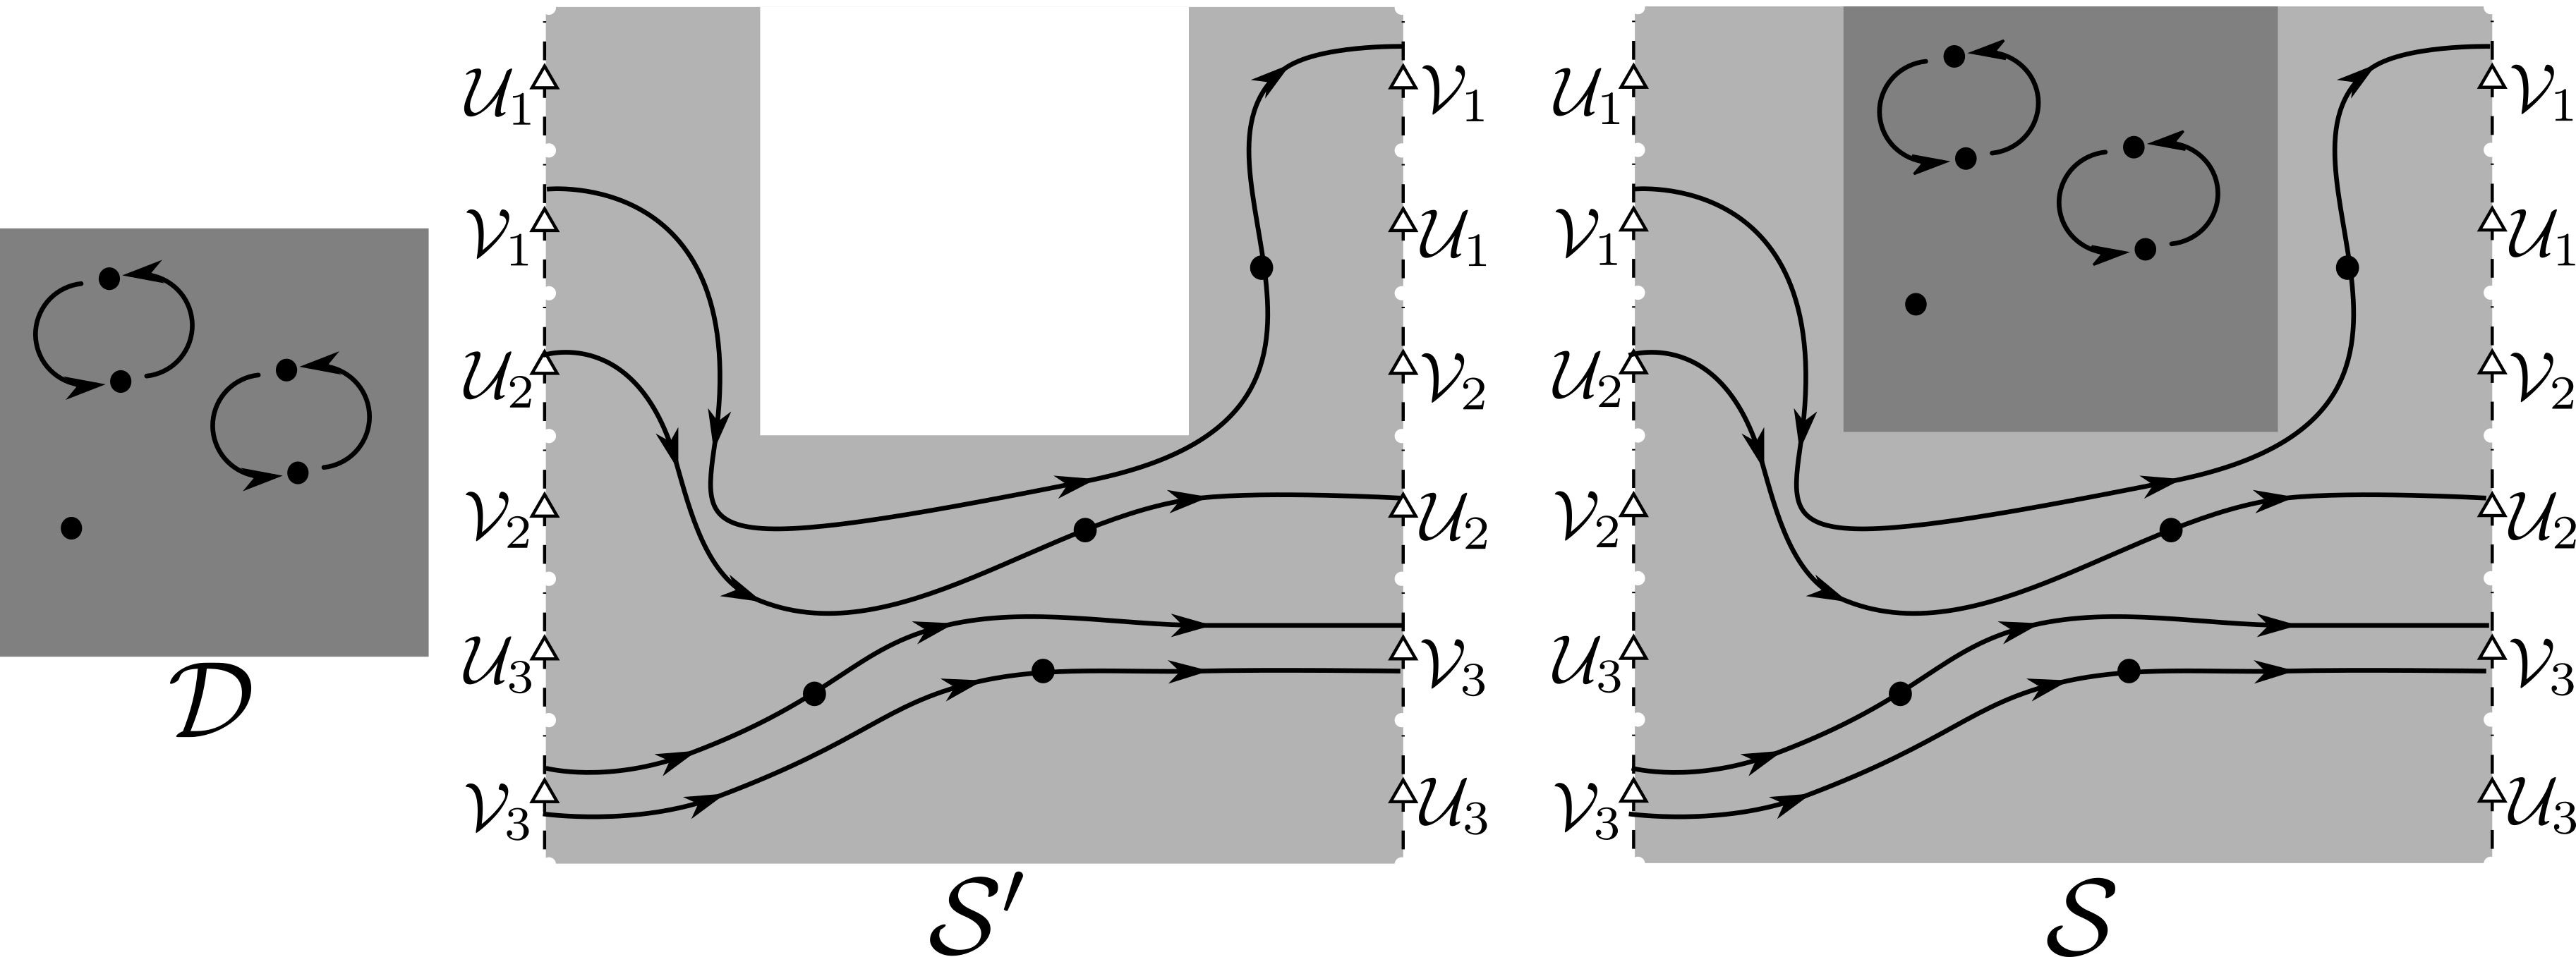
\includegraphics[scale=0.65]{figures/axb.pdf}
 \caption{From left to right, the class $[a]=\epsilon\cdot(Q\epsilon)^2\in H_2(C_5(\D))$;
 the class $[b]=\v_1\cdot\u_2\cdot\v_3^2\in H_4(C_4(\S'))$; and the product class
 $\mu_*([a]\otimes[b])\in H_6(C_9(\S))$.}
\label{fig:axb}
\end{figure}

Then $[a]\otimes [b]$ is a generator of $H_{p-l}(C_p(\D))\otimes H_{m-p}(C_{m-p}(\S'))$,
by the K\"unneth formula, and we are interested in the homology class $\mu_*([a]\otimes [b])$.

There is one such
class for any choice of $[a]$ and $[b]$ as above, that is, for any choice of
$p$, $\ualpha$, $\uu$ and $\uv$ satisfying the conditions
$l=\sum_{j\geq 0}\alpha_j$, $p=\sum_{j\geq 0}\alpha_j2^j$ and $(m-p)=\sum_{i=1}^g(u_i+v_i)$, where
we use the notation above.

We want to show that the collection of all the corresponding classes of the form $\mu_*([a]\otimes [b])$
gives a basis for $H_{m-l}(\cms)$.

We will study
the intersection of $\mu_*([a]\otimes [b])$ with cohomology classes of $\cms$ represented by
generalised symmetric chains in $\cms^{\infty}$.

% $[a]\otimes [b]$ has a dual class in $\tH_{p-l}(C_p(\D)^{\infty})\otimes \tH_p(C_{m-p}(\S')^{\infty})$
% represented by the product of generalised symmetric chains
% \[
%  (\alpha_j)_j\otimes (p,(u_i,v_i)_{i\leq g}).
% \]
% If $\tup=(l,(x_i)_{i\leq l})$ is a tuple such that $e^{\tup}$ appears in the symmetric
% chain $(\alpha_j)_j$, and if $\tup'=(0,(u_i,v_i)_{i\leq g})$ is the only tuple such that
% $e^{\tup'}$ appears in the generalised symmetric chain $(p,(u_i,v_i)_{i\leq g})$, then
% the product $e^{\tup}\times e^{\tup'}\subset C_p(\D)\times C_{m-p}(\S')\subset\cms$ is
% contained in the closure of the generalised symmetric chain $e^{\tup}$, where...



% If $p<p'$ then
% the \emph{geometric} intersection between the cycle $|p',(\alpha'_j),(u'_i,v'_i)|$
% in $\cms^{\infty}$ and the cycle $\mu_*(a\otimes b)$ in $\cms$ is empty: indeed the first cycle is supported
% on $\infty\in\cms^{\infty}$ and on configurations where at least $p'$ points lie in the union
% $\bigcup_i(\U_i\cup\V_i)\subset\S'$,
% whereas the second cycle is supported on configurations where at least $m-p$ points lie
% inside $\D$. The algebraic intersection between the homology classes $\mu_*([a]\otimes [b])$
% and $[p',(\alpha'_j),(u'_i,v'_i)]$ is therefore also zero.
% 
% Consider now the case $p=p'$.

To compute the algebraic intersection
between $\mu_*([a]\otimes [b])$ and $[\kappa(p',\ualpha',\uu',\uv')]$ we
consider the map
\[
 \mu^{\infty}\colon \cms^{\infty}\to \pa{C_p(\D)\times C_{m-p}(\S')}^{\infty}
\]
which collapses to $\infty$ the complement in $\cms^{\infty}$ of the open submanifold $C_p(\D)\times C_{m-p}(\S')$.

By Poincaré-Lefschetz duality, the map $\mu^{\infty}_*$ in reduced homology corresponds to the cohomology map
\[
 \mu^*\colon H^*(\cms)\to H^*(C_p(\D)\times C_{m-p}(\S'))=H^*(C_p(\D))\otimes H^*(C_{m-p}(\S')).
\]

We give $\pa{C_p(\D)\times C_{m-p}(\S')}^{\infty}$ the cell complex structure of the smash product
$C_p(\D)^{\infty}\wedge C_{m-p}(\S')^{\infty}$. Here $C_p(\D)^{\infty}$ is given the cell structure of $C_p((0,1)^2)^{\infty}$
coming from the natural identification $\D=]1/4,3/4[\times]1/2,1[\cong]0,1[^2$, which is obtained by rescaling
and translating. Moreover we choose any diffeomorphism $\mrS'\cong\mrS$ that restricts to the identity
on all $\U_i$'s and $\V_i$'s, and give $C_{m-p}(\S')^{\infty}$ the cell structure of $C_{m-p}(\S)^{\infty}$.

Recall that $\cms^{\infty}$ can be filtered according to the norm of cells: a cell $e^{\tup}$ associated with
the tuple $\tup=(l,\ux,\uu,\uv)$ has norm $\sum_{i=1}^l x_i$, and the norm is weakly decreasing along boundaries.
In the previous section we just considered
the associated filtration of the reduced chain complex $\tCh_*(\cms^{\infty})$, whereas now we
consider the closed subcomplex $F_p\cms^{\infty}\subset\cms^{\infty}$, which is the union
of all cells of norm $\leq p$.

The crucial observation is that $\mu^{\infty}$ restricts to a cellular map 
\[
F_p\cms^{\infty}\to \pa{C_p(\D)\times C_{m-p}(\S')}^{\infty}.
\]

To see this, fix a tuple $\tilde{\tup}=(\tilde{l}, \tilde{\ux},\tilde{\uu},\tilde{\uv})$ of norm $\tilde{p}\leq p$
and of dimension $\tilde{l}+m$, and
consider the open cell
cell $e^{\tilde{\tup}}\subset F_p\cms^{\infty}$.

If $\tilde{p}<p$, then
$e^{\tilde{\tup}}\cap (C_p(\D)\times C_{m-p}(\S'))$ is empty. If $\tilde{p}=p$, then
\[
e^{\tilde{\tup}}\cap (C_p(\D)\times C_{m-p}(\S'))=e^{\tup'}\times e^{\tup''},
\]
where $\tup'=(\tilde{l},\tilde{\ux})$ and $\tup''=(0,\tilde{\uu},\tilde{\uv})$.

Therefore
$\mu^{\infty}(e^{\tilde{\tup}})$ is $\set{\infty}$ in the first case, and in the second case it
is contained in the union $\set{\infty}\cup e^{\tup'}\times e^{\tup''}$, which is also
contained in the $(\tilde{l}+m)$-skeleton of $\pa{C_p(\D)\times C_{m-p}(\S')}^{\infty}$.

% We replace the map $\mu^{\infty}$ by a cellular approximation that agrees with it on the $p$-skeleton,
% and by abuse of notation we still call $\mu^{\infty}$ the new map.
% 
Consider now the generalised symmetric chain $\kappa(p',\ualpha',\uu',\uv')$ representing
a class in $\tH_{m+l}(\cms^{\infty})=H^{m-l}(\cms)$, with $\ualpha'=(\alpha'_j)_{j\geq 0}$,
$\uu'=(u_1,\dots,u'_g)$ and $\uv'=(v'_1,\dots,v'_g)$; in particular $l=\sum_{j\geq 0}\alpha'_j$.
Suppose moreover $p'\leq p$.

If $p'<p$, the previous argument shows that $\mu^{\infty}_*\pa{\kappa(p',\ualpha',\uu',\uv')}=0$
in the reduced cellular chain complex,
and in particular the corresponding homology class is mapped to zero.

Suppose now $p'=p$: then the previous argument shows that
the homology class $[\kappa(p',\ualpha',\uu',\uv')]\in \tH_{m+l}(\cms^{\infty})$
is mapped along $\mu^{\infty}_*$ to the class
\[
[\kappa(\ualpha')]\otimes [\kappa(\uu',\uv')]\in\tH\pa{C_p(\D)^{\infty}\wedge C_{m-p}(\S')^{\infty}}.
\]
Indeed each tuple $\tup$ in the cycle $\kappa(p',\ualpha',\uu',\uv')|$ is mapped by $\mu^{\infty}_*$
to a corresponding pair of tuples $\tup'\otimes\tup''$ in the cycle $\kappa(\ualpha')\otimes \kappa(\uu',\uv')$,
so even at the level of chains we have
\[
\mu^{\infty}_*\pa{\kappa(p',\ualpha',\uu',\uv')}=\kappa(\ualpha')\otimes \kappa(\uu',\uv').
\]

We can now compute the algebraic intersection of $\mu_*([a]\otimes [b])$ with
the cohomology class $[\kappa(p',\ualpha',\uu',\uv')]$ as the algebraic intersection between
$[a]\otimes [b]$ and $\mu^{\infty}_*\pa{[\kappa(p',\ualpha',\uu',\uv')]}$.

For $p'<p$ the previous argument show that this intersection is zero.

For $p'=p$ the intersection between
$[a]\otimes [b]$ and $\mu^{\infty}_*([\kappa(p,\ualpha',\uu',\uv')])=[\kappa(\ualpha')]\otimes [\kappa(\uu',\uv')]$
is $1\in\Z_2$ exactly when $\ualpha=\ualpha'$, $\uu=\uu'$ and $\uv=\uv'$; otherwise it is $0$.

To finish the proof we consider the collection of all strings of the form
\[
\pa{p,\ualpha=(\alpha_j)_{j\geq 0},\uu=(u_1,\dots,u_g),\uv=(v_1,\dots,v_g)}
\]
satisfying $l=\sum_j\alpha_j$,$p=\sum_j \alpha_j2^j$ and $(m-p)=\sum_i(u_i+v_i)$;
we choose a total order on the set of these strings,
such that the parameter $p$ is weakly increasing along this order; we associate
to each string its corresponding class in $H_{m-l}(\cms)$ of the form $\mu_*([a]\otimes [b])$ and its
corresponding class $[\kappa(p,\ualpha',\uu',\uv')]\in\tH_{m+l}(\cms^{\infty})$.

Then the matrix of algebraic intersections between these two sets of
classes is an upper-triangular matrix
with $1$'s on the diagonal, and in particular
it is invertible. This shows that the set of classes of the form $\mu_*([a]\otimes [b])$
is a basis for $H_{m-l}(\cms)$.

% 
% 
% 
% , and let $e^{\tup}$
% be one of the cells appearing in this generalised symmetric chain, with
% $\tup=(l,(x_i)_{i\leq l}, (u_i,v_i)_{i\leq g})$, and consider the restriction
% of $\mu^{\infty}\colon\cms^{\infty}\to \pa{C_{m-p}(\S')\times C_p(\D)}^{\infty}$
% to $e^{\tup}\subset\cms^{\infty}$
% 
% If $p\neq p'$, the whole cell $e^{\tup}$ is mapped
% to $\infty$: indeed if $p<p'$, then a configuration in $e^{\tup}$ contains
% at least $p'$ points inside $\S'$, so it cannot lie in $C_p(\D)\times C_{m-p}(\S')$;
% if $p'<p$ then a configuration in $e^{\tup}$ contains at least $m-p$ points 
% 
% 
% then the algebraic
% intersection between $(p',(u'_i,v'_i),(\alpha'_j))$ and $\mu_*(a\otimes b)$ is $0\in\Z_2$,
% unless $p=p'$, $\alpha_j=\alpha'_j$ for all $j$, and $u_i=u'_i$ and $v_i=v'_i$ for all $1\leq i\leq g$.
% 
% Indeed the generalised symmetric chain $(p',(u'_i,v'_i),(\alpha'_j))$ hits only configurations
% in $\cms$ where for all $1\leq i\leq g$ at least $u'_i$ points lie on $\U_i$ and at least $v'_i$
% points lie on $\V_i$
\end{proof}

One could expect that the basis given by classes of the form $[a]\otimes [b]\in H_{m-l}(\cms)$
is also \emph{dual} to the basis of classes $[\kappa(p,\ualpha,\uu,\uv)]\in \tH_{m+l}(\cms^{\infty})$, i.e., the
matrix considered in the end of the previous proof is not only upper-triangular but also
diagonal. This is however not true, as the following example shows.

Let $g=1$, $m=2$, $p=1$, $p'=2$ and consider the classes $[a]=\epsilon\in H_0(C_1(\D))$,
$[b]=\u_1\in \H=H_1(C_1(\S'))$. Moreover let the generalised symmetric chain
$\kappa(p',\ualpha',\uu',\uv')$ be defined by
$\ualpha'=(\alpha'_j)_{j\geq 0}$ with $\alpha'_1=1$ and all other $\alpha_j=0$, $\uu'=(u'_1=0)$
and $\uv'=(v'_1=0)$.

Represent $[a]$ by a point in $a\in\D$, for example
the point $(1/2,3/4)$; represent $[b]$ by a simple closed curve $b\subset\S'$
that intersects only once, transversely, the vertical segment passing through $a$, i.e.
$\set{1/2}\times]0,1[$. See Figure \ref{fig:counterexample}.

\begin{figure}\centering
 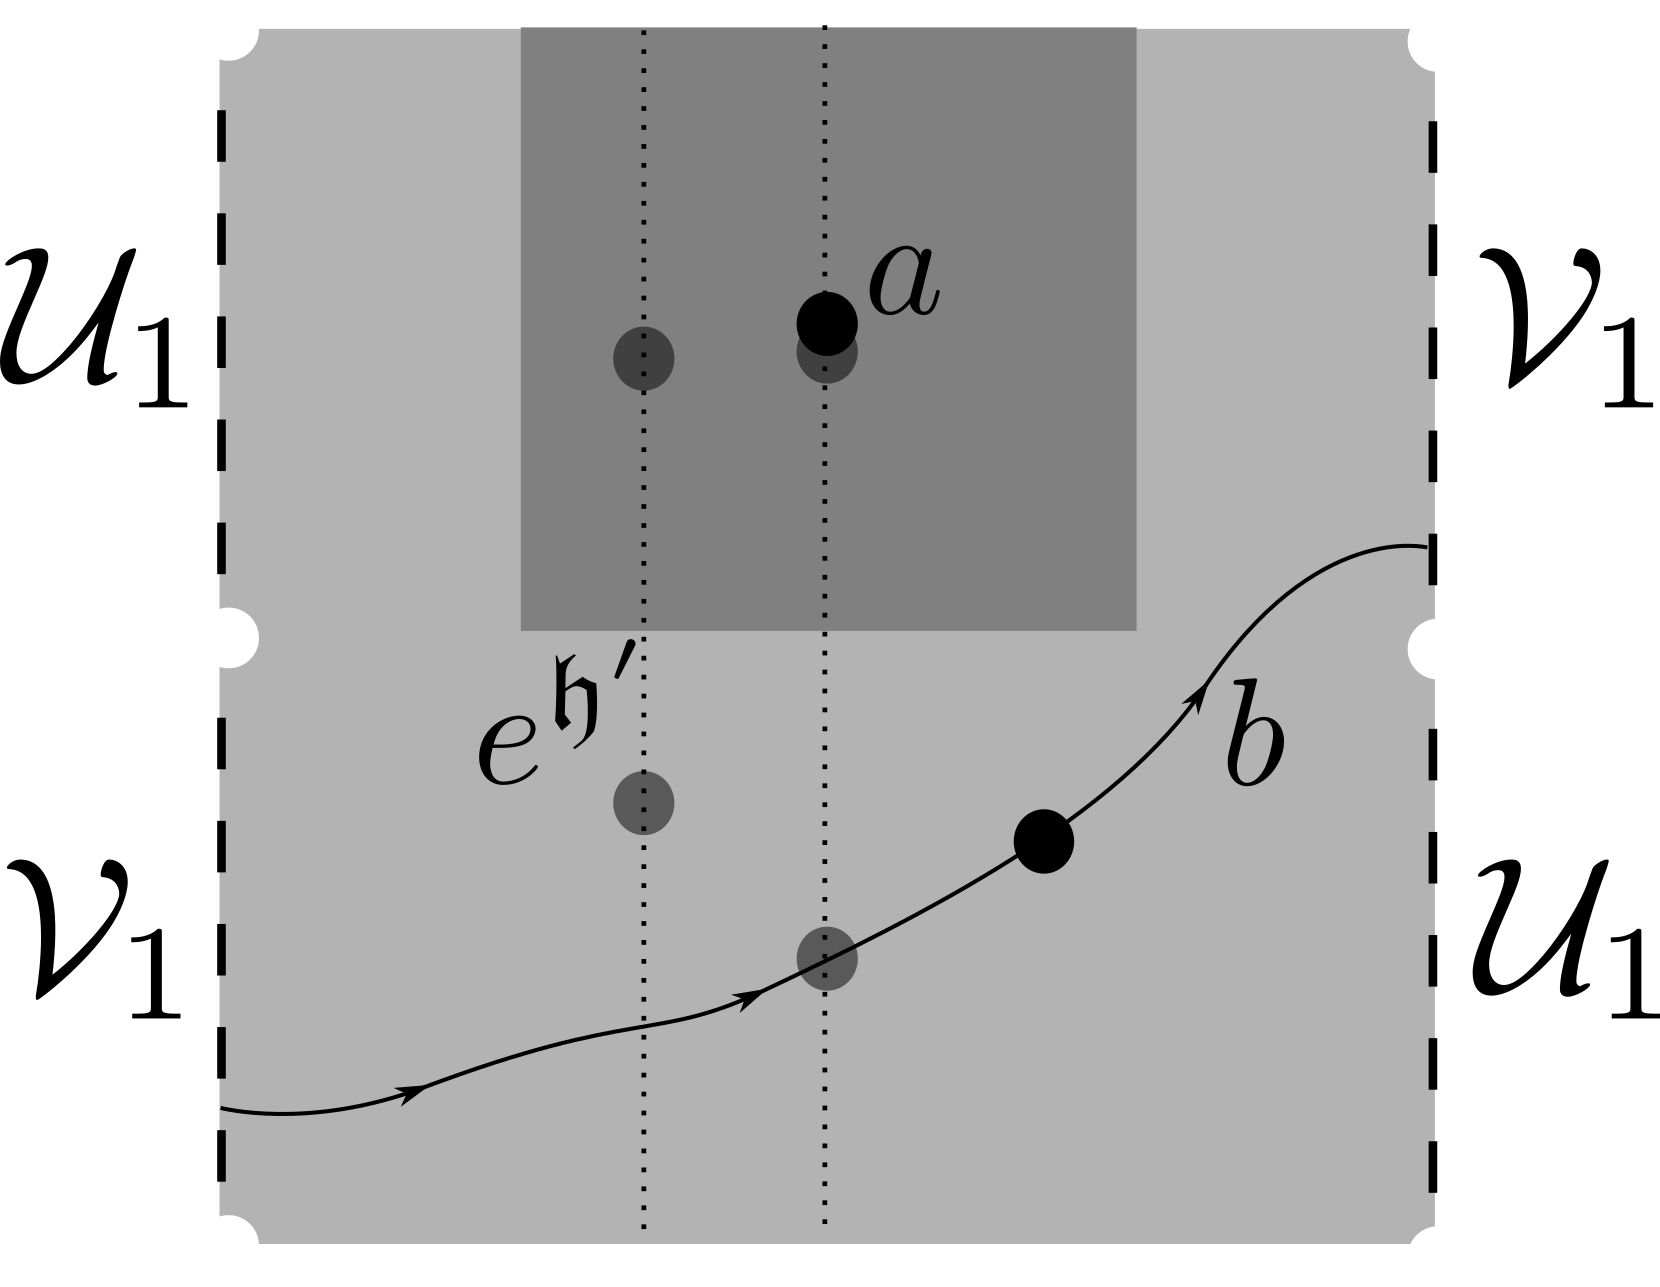
\includegraphics[scale=0.6]{figures/counterexample.pdf}
 \caption{$\mu_*(a\otimes b)$ and $e^{\tup'}$ intersect once, transversely inside $C_2(\S)$.}
\label{fig:counterexample}
\end{figure}

Then the cycle $\kappa(p',\ualpha',\uu',\uv')$ consists uniquely of one tuple
\[
\tup'=(1,\ux'=(x'_1=2),\uu'=(u'_1=0),\uv'=(v'_1=0)).
\]
The corresponding cell $e^{\tup'}$ intersects once, transversely,
the cycle $\mu_*(a\otimes b)$, which is represented by the curve of configurations of two
points in $\mrS$, one of which is fixed at $a$ whereas the other runs along $b$:
there is exactly one position on $b$ lying under $a$.

Hence the algebraic intersection between these two classes is $1$, and since $p'>p$
this is an entry strictly above the diagonal in the matrix considered in the proof
of Lemma \ref{lem:oplussplitting}.

The proof of Theorem \ref{thm:Hbms*as*ggrep} can be easily generalised to surfaces
with more than one boundary component. Let $\Sigma_{g,n}$ be a surface of genus
$g$ with $n\geq 1$ parametrised boundary components and let $\Gamma_{g,n}$ be
the group of connected components of the topological group
$\Diff(\Sigma_{g,n};\partial\Sigma_{g,n})$:
then there is an isomorphism of bigraded $\Z_2$-representations
\begin{equation}
\label{eq:sgn}
\bigoplus_{m\geq 0}H_*\pa{C_m(\Sigma_{g,n})}\simeq \Z_2\left[Q^j\epsilon\,|\, j\geq 0\right]\otimes\Sym_{\bullet}(H_1(\Sigma_{g,n})),
\end{equation}

where the action of $\Gamma_{g,n}$ on the right-hand side is induced by the natural
action on $H_1(\Sigma_{g,n})$.

For $n\geq 2$ the intersection form on the vector space $H_1(\Sigma_{g,n})$
is \emph{degenerate}, but it is still invariant under the action of
$\Gamma_{g,n}$, so there is still a map from $\Gamma_{g,n}$ to the subgroup
of $GL_{2g+n-1}(\Z_2)$ fixing this bilinear form, and in this sense we can say
that the representation in \eqref{eq:sgn} is \emph{symplectic}.

The proof of the isomorphism \eqref{eq:sgn} is almost verbatim the same; the main difference is in the construction of the
model $\T(\Sigma_{g,n})$ for $\mathring{\Sigma}_{g,n}$: we divide the
vertical segments $\set{0,1}\times[0,1]\subset[0,1]^2$
into $2g+n-1$ equal parts, that we call $I_i^l$ and $I_i^r$ according to their order;
we identify, for each $i>2g$, the interval $I_i^l$ with the interval $I_i^r$;
the other couples of intervals, yielding the genus, are identified just as before.

One can further generalise to non-orientable surfaces with non-empty boundary: it suffices,
in the above construction, to glue some of the intervals $I_i^l$ and $I_i^r$ reversing their
orientation. We leave all details of these generalisations to the interested reader.

\section{Proof of Theorem \ref{thm:main}}
We will prove Theorem \ref{thm:main} by induction on $m$.
The case $m=0$ is trivial.

For all $m\geq 0$ we let $E(m)$ be the Leray-Serre spectral sequence associated with
the bundle \eqref{eq:BirmanbundleD}: its second page has the form
\[
 E(m)^2_{k,q}=H_k(B\Diff(\S;\partial\S\cup\D);H_q(\cms))=H_k(\gg;H_q(\cms)).
\]
From Theorem \ref{thm:Hbms*as*ggrep} we know that this spectral sequence is concentrated
on the rows $q=0,\dots, m$.

We want to prove the vanishing of all differentials appearing in the pages
$E(m)^r$ with $r\geq 2$; the $r$-th differential takes the form
\[
 \partial_r\colon E(m)^r_{k,q}\to E(m)^r_{k-r,q+r-1}.
\]
In particular any differential $\partial_r$ exiting from the row $q=m$ is trivial,
because it lands in a higher, hence trivial row.

Fix now $q=m-l<m$, in particular $l\geq 1$; by Theorem \ref{thm:Hbms*as*ggrep}, and
in particular by Lemma \ref{lem:oplussplitting}, we have a splitting of $H_k(\gg;H_{m-l}(\cms))$ as
\begin{equation}
\label{eq:Hksplitting}
 \bigoplus_{p=l}^m H_k\pa{\gg;\mu_*\pa{H_{p-l}(C_p(\D))\otimes H_{m-p}(C_{m-p}(\S'))}}.
\end{equation} 
We fix now $l\leq p\leq m$ and show the vanishing of all differentials $\partial_r$ exiting from the
summand with label $p$ in the previous equation.

Consider the map $\mu^{\cF}$ from Definition \ref{defn:universalSbundle} as a map of
bundles over the space $B\Diff(\S;\partial\S\cup\D)$:
\[
 \mu^{\cF}\colon C_p(\D)\times C_{m-p}(\cF_{\S'})\to C_m(\cF_{\S,\D}).
\]
Note that the first bundle $C_p(\D)\times C_{m-p}(\cF_{\S'})\to B\Diff(\S;\partial\S\cup\D)$
is the product of the space $C_p(\D)$ with the bundle $C_{m-p}(\cF_{\S'})\to B\Diff(\S;\partial\S\cup\D)$;
therefore the spectral sequence associated with $C_p(\D)\times C_{m-p}(\cF_{\S'})$ is isomorphic,
from the second page on, to the tensor product
of $H_*(C_p(\D))$ and the spectral sequence associated with the bundle $C_{m-p}(\cF_{\S'})$; the
latter spectral sequence is isomorphic, in our notation, to the spectral sequence $E(m-p)$.
In particular $\mu^{\cF}$ induces a map of spectral
sequences
\[
\mu^{\cF}_*\colon H_*(C_p(\D))\otimes E(m-p)\to E(m);
\]
that in the second page, on the $(m-l)$-th row and $k$-th column, restricts to
the inclusion of one of the direct summands in equation \eqref{eq:Hksplitting}:
\[
H_k\pa{\gg;\mu_*(H_{p-l}(C_p(\D))\otimes H_{m-p}(C_{m-p}(\S')))}\subset H_k\pa{\gg;H_{m-l}(\cms)}.
\]

In particular if we prove the vanishing of all differentials $\partial_r$
% exiting from the summand
% $H_k\pa{\gg;H_{p-l}(C_p(\D))\otimes H_{m-p}(C_{m-p}(\S'))}$
in the first spectral sequence, then also all differentials
$\partial_r$ exiting from this direct summand in the
second spectral sequence $E(m)$ must vanish.

% We observe that there is an isomorphism
% \[
%  H_k\pa{\gg;H_{p-l}(C_p(\D))\otimes H_{m-p}(C_{m-p}(\S'))}\simeq H_{p-l}(C_p(\D))\otimes H_k\pa{\gg; H_{m-p}(C_{m-p}(\S'))};
% \]
The differentials in the spectral sequence $H_*(C_p(\D))\otimes E(m-p)$
are obtained by tensoring the identity of $H_*(C_p(\D))$ with the differentials
of the spectral sequence $E(m-p)$; as $p\geq l\geq 1$ we know by inductive hypothesis
that the latter vanish. Theorem \ref{thm:main} is proved.

One can generalise Theorem \ref{thm:main} to orientable or non-orientable
surfaces with non-empty boundary, following the generalisation
of Theorem \ref{thm:Hbms*as*ggrep} discussed at the end of section \ref{sec:Actiongg}.

\section{Computation in genus one}
We can apply the results from the previous sections, in particular theorems \ref{thm:main}
and \ref{thm:Hbms*as*ggrep}, to compute the groups $H_*(\gone^m)$ explicitly.

Recall that $\gone$ is generated by two Dehn twists $\tu$ and $\tv$ about two simple
closed curves $\u,\v\subset\Sigma_{1,1}$ that intersect once transversely; a presentation
for $\gone$ is given by
\[
 \gone=\left<\tu,\tv\, |\, \tu\tv\tu=\tv\tu\tv \right>
\]
and therefore $\gone$ is isomorphic to the braid group on three strands $\beta_3=\beta_3(\D)$.

\section{A rational counterexample}
In this section we prove that a statement as in theorem \ref{thm:Hbms*as*ggrep}
cannot hold if we consider homology with coefficients in $\Q$. We still don't know
if the analogue of theorem \ref{thm:main} holds in homology with coefficients in $\Q$
or in fields of odd characteristic.

We recall that $H_*(C_m(\Sigma_{g,1});\Q)$ has been computed \emph{as a bigraded $\Q-$vector space}
by B\"odigheimer, Cohen and Milgram in \cite{BCM}, and more recently by Knudson in \cite{Knudson}. A description of
these homology groups as a
$\gg-$representation seems to be still missing in the literature.

We will prove the following theorem:
\begin{thm}
 \label{thm:counterexample}
 Let $g\geq 2$ and $m\geq 2$; then $H_2(C_2(\Sigma_{g,1});\Q)$ is not a symplectic
 representation of $\gg$.
\end{thm}
\begin{proof}
 Let again $\S=\Sigma_{g,1}$. We will use the following strategy:
 \begin{itemize}
  \item we define a homology class $[a]\in H_2(C_2(\S);\Q)$ represented by a cycle $a$;
  \item we prove that $[a]\neq 0$ by computing the algebraic intersection of
  $[a]$ with a homology class
  in $\tH_2(\cms^c;\Q)$; here it is worth stressing that the manifold
  $\cms$ is orientable: therefore we can apply Poincaré-Lefschetz duality
  also with rational coefficients;
  \item we define another homology class $[b]\in H_2(\cms;\Q)$ and show that
  $[b]$ is mapped to $[b]+2[a]$ by some element in the Torelli group $\mathcal{I}_{g,1}$.
 \end{itemize}
Recall that the Torelli group $\mathcal{I}_{g,1}$ is the kernel of the surjective homomorphism
$\gg\to Sp_{2g}(\Z)$; if an element of the Torelli group acts non-trivially on
some class in $H_2(C_2(\S);\Q)$, then this is not a symplectic representation of $\gg$.

We consider again $\T(\S)$ as model for $\mrS$. Let $c$ be an simple closed curve
representing the homology class $\u_1$, and assume that $c$ intersects $\U_1$ once
transversely and is disjoint from all other $\U_i$'s and from all $\V_i$'s. Let $c'$
be a parallel copy of $c$.

We consider the torus $a=c\times c'$ of configurations in $C_2(\S)$ having one point lying on $c$ and
one lying on $c'$: by abuse of notation, denote also one of its fundamental cycles by $a$
(there are two possible choices, corresponding to the two possible orientations of $a$).

Let $\tup=(0,(u_i,v_i))$ with $u_1=2$ and all other $u_i$'s, as well as all $v_i$'s, equal to zero.
Then the map
\[
\phi_{\tup}\colon (\Delta^{\tup},\partial\Delta^{\tup})\to (C_2(\S)^c,\infty)
\]
maps the fundamental class in $H_2(\Delta^{\tup},\partial\Delta^{\tup};\Q)$ to a homology
class in $\tH_2(C_2(\S)^c;\Q)$.
% ; if we see $e^{\tup}$ as a properly embedded, orientable submanifold
% of $C_2(\S)$, then we are just considering its fundamental class $[e^{\tup}]\in H_2(C_2(\S)^c)$.

The cell $e^{\tup}$ intersects once, transversely the torus $a$, therefore the
algebraic intersection $[a]\cap[e^{\tup}]$ is $\pm 1$,
where the signs depends on how we have chosen orientations on $a$, $e^{\tup}$ and $C_2(\S)$ itself;
in particular $[a]\neq 0$.

The action of $\gg$ on isotopy classes of simple closed curves is transitive, so we can repeat
the construction of the torus $a$ with any other copy of parallel, non-separating simple closed curves
$c$ and $c'$, and the resulting class $[a]$ will always be non-trivial in $H_2(C_2(\S);\Q)$.

See figure \ref{fig:rational} to visualize the following discussion.
Let $d$ and $d'$ be disjoint, non-separating simple closed curves such that
cutting $\S$ along $d$ and $d'$ we obtain a subsurface $\S'\simeq\Sigma_{1,2}$ of genus 1, with boundary
components $d$ and $d'$ (here we need that the genus of $\S$ is at least 2);
suppose moreover that $c$ is a non-separating simple closed curve in $\S'$,
and let $c',c''$ be two parallel copies of $c$ in $\Sigma_{1,2}$, one on each side of a small tubular
neighborhood of $c$.
Then $d,d',c',c''$ are the boundary of a subsurface $\S''\simeq\Sigma_{0,4}\subset\S'$.
Orient all curves $d,d',c,c',c''$ in such a way that the following equalities hold:
\begin{itemize}
 \item $[d]=[d']\in H_1(\S;\Q)$, as witnessed by the subsurface $\S'$;
 \item $[c]=[c']=[c'']\in H_1(\S;\Q)$;
 \item $[d]-[d']+[c']-[c'']=0\in H_1(\S\setminus c;\Q)$, as witnessed by the subsurface $\S''$.
\end{itemize}

\begin{figure}\centering
 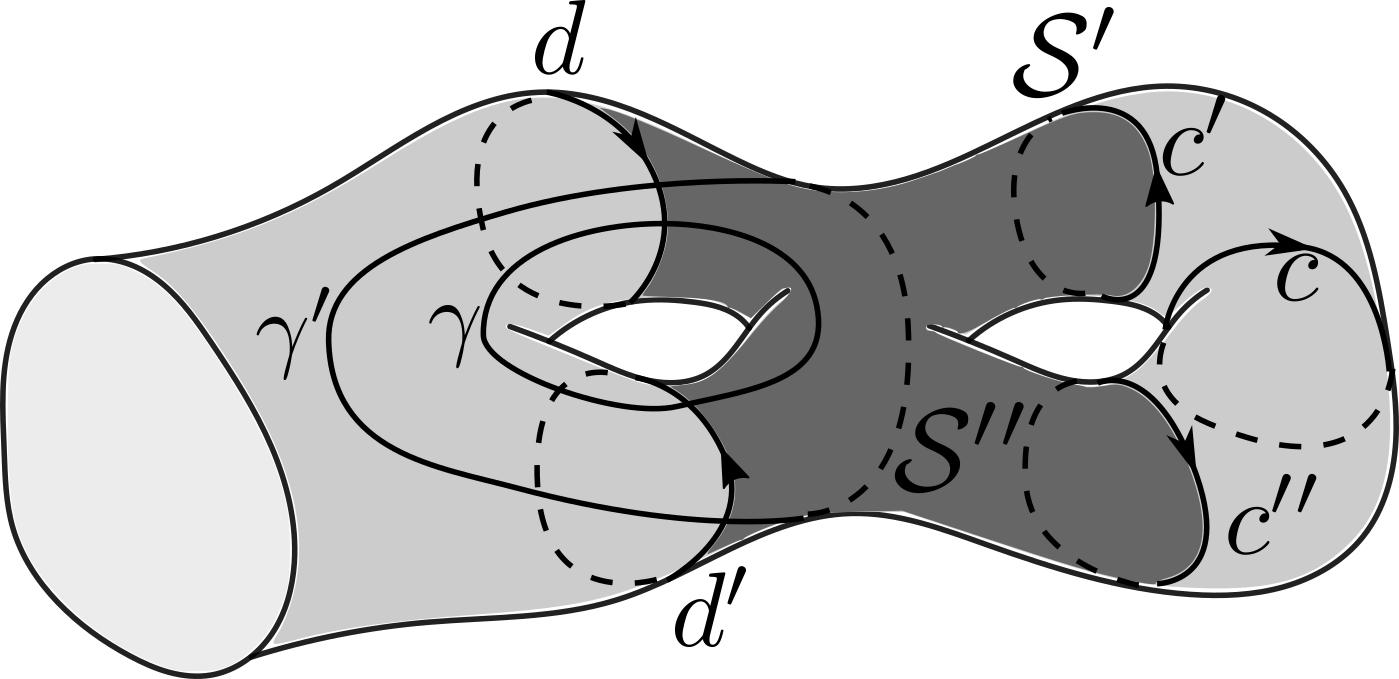
\includegraphics[scale=1.0]{figures/rational.png}
 \caption{The curves $d,d',c,c',c'',\gamma,\gamma''$ and the subsurfaces $\S',\S''$.}
\label{fig:rational}
\end{figure}

The four tori $c\times c'$, $c\times c''$, $c\times d$ and $c\times d'$ are contained in $C_2(\S)$
and the equality
\[
 [c\times d]-[c\times d']+[c\times c']-[c\times c'']=0\in H_2(C_2(\S))
\]
holds, as witnessed by the homology $c\times \S''\subset C_2(\S)$.

Moreover the classes $[c\times c']$ and $-[c\times c'']$ are \emph{equal}:
indeed there is an isotopy of $\S$ mapping $c$ to $c'$ and $c''$ to $c$,
as oriented curves; the class $[c\times c'']$ is mapped to the class $[c'\times c]=-[c\times c']$.

Let again $a=[c\times c']$ and let $b=[c\times d]$: then the class $b'=[c\times d']$
is equal to $b+2a\in H_2(C_2(\S);\Q)$.

Consider now an element of the Torelli group that fixes $c$ and maps $d$ to $d'$ preserving
the orientation, for example the bounding pair $D_{\gamma}\circ D_{\gamma'}^{-1}$, where
$\gamma$ and $\gamma'$ are represented in figure \ref{fig:rational}:
then the class $b$ is mapped to $b'=b+2a\neq b$.
\end{proof}

The previous proof works word by word if we replace $\Q$ by any field of odd characteristic. Moreover
all the arguments in the previous proof can be adapted to show that $H_*(F_2(\S);\mathbb{F})$ is
not a symplectic representation of $\gg$, where $F_2(\S)$ is the ordered configuration space
and $\mathbb{F}$ is \emph{any} field, including $\Z_2$. The result of theorem \ref{thm:Hbms*as*ggrep}
is peculiar of unordered configurations and characteristic 2.

\input{Conclusions.tex}

\bibliography{Bibliography.bib}{}
\bibliographystyle{plain}

\end{document}




